\documentclass[
    11pt,
    a4paper,
    sfdefaults=false,
    toc=chapterentrywithdots,
    twoside,openright,
    titlepage,
    parskip=half,
    headings=normal,  % reduces heading size
    listof=totoc,
    bibliography=totoc,
    index=totoc,
    captions=tableheading,  % caption below table
    chapterprefix,
    listof=flat,
    final,
    openany
]{scrbook}


% details about your thesis
\newcommand{\titel}{Automatische Generierung von themenspezifischen Podcasts aus einer großen Audiodatenbank}
\newcommand{\artderarbeit}{Bachelorarbeit}  % {Bachelorarbeit,Masterarbeit}
\newcommand{\autor}{Vincent Neumann}
\newcommand{\studiengang}{Medieninformatik}  % {Informatik,Wirtschaftsinformatik,Medieninformatik}
\newcommand{\matrikelnr}{358\,5287}
\newcommand{\erstgutachter}{Prof.\,Dr.~Florian Gallwitz}
\newcommand{\zweitgutachter}{Prof.\,Dr.~Anna Kruspe}
\newcommand{\betreuer}{Florian Thoma}
\newcommand{\unternehmen}{Public Value Technologies GmbH}
\newcommand{\logo}{figures/TH-Nuernberg-RGB.png}
\newcommand{\keywords}{hot, fuzz}
 

% custom head and foot
\usepackage[automark]{scrlayer-scrpage}
\pagestyle{scrheadings}
\ihead{\headmark}
\chead{}
\ohead{\pagemark}
\renewcommand*\chaptermarkformat{\chapappifchapterprefix{\ }% 
  \thechapter.\enskip}

\RedeclareSectionCommand[tocindent=0pt]{section}
\RedeclareSectionCommand[tocindent=0pt]{subsection}
%\RedeclareSectionCommand[tocnumwidth=70pt]{chapter}

\usepackage{scrhack}

% other packages
\usepackage[utf8]{inputenc}
\usepackage[T1]{fontenc}
\usepackage{lmodern,relsize,textcomp,csquotes}
\usepackage{amsmath,amsfonts}
\usepackage[english, ngerman]{babel}  % flip for German thesis
\usepackage[final]{graphicx}
\usepackage{setspace,geometry,xcolor}
\usepackage{makeidx}
\usepackage{paralist,ifthen,todonotes}
\usepackage{url}
\usepackage[toc]{glossaries}
\usepackage{pdfpages}
\usepackage{amsmath}

% table setup
\usepackage{longtable}
\usepackage{array}
\usepackage{ragged2e}
\usepackage{lscape}

\usepackage{xurl}

% \def\UrlBreaks{\do\/\do-}s

% pdf hyperref
\usepackage[
    bookmarks=true,
    bookmarksopen=true,
    bookmarksnumbered=true,
    bookmarksopenlevel=1,
    pdftitle={\titel},
    pdfauthor={\autor},
    pdfcreator={\autor},
    pdfsubject={\titel},
    pdfkeywords={\keywords},
    pdfpagelabels=true,
    colorlinks=true,
    linkcolor=red,
    urlcolor=magenta,
    anchorcolor=black,
    citecolor=cyan,
    filecolor=magenta,
    menucolor=red,
    plainpages=false,
    hypertexnames=true,
    linktocpage=true,
]{hyperref}

% \PassOptionsToPackage{hyphens}{url}\usepackage{hyperref}

% biblatex
% \usepackage[backend=biber, style=authoryear]{biblatex}
\usepackage{biblatex} 
% \addbibresource{literatur.bib}

% configure your listings style
\usepackage{listings}
\lstset{
	tabsize=3,
	extendedchars=true,
	frame=single,
	showstringspaces=true,
	numbers=left,
	numberstyle=\small,
	breakautoindent=true
}

% page setup
% \setlength{\topskip}{\ht\strutbox}
\geometry{paper=a4paper,left=2.5cm,top=3.0cm,bindingoffset=.8cm}
\onehalfspacing
\frenchspacing
\clubpenalty = 10000
\widowpenalty = 10000 
\displaywidowpenalty = 10000

% some commands
\newcommand{\ua}{\mbox{u.\,a.\ }}
\newcommand{\zB}{\mbox{z.\,B.\ }}
\newcommand{\dahe}{\mbox{d.\,h.,\ }}
\newcommand{\bzw}{\mbox{bzw.\ }}
\newcommand{\bzgl}{\mbox{bzgl.\ }}
\newcommand{\eg}{\mbox{e.\,g.\ }}
\newcommand{\ie}{\mbox{i.\,e.\ }}
\newcommand{\wrt}{\mbox{w.\,r.\,t.\ }}
\newcommand{\etal}{\mbox{\emph{et.\,al.\ }}}
\newcommand{\myfigure}[3]{%
    \begin{figure}[h]
        \centering
        \includegraphics[width=\linewidth]{figures/#1}
        \caption{#2}
        \label{fig:#3}
    \end{figure}
}
\newcommand{\qt}[1]{\glqq #1\grqq}


% TODO remove if not needed...
\usepackage{blindtext}

% load glossary entries
\makenoidxglossaries
\loadglsentries{glossary}

\addbibresource{literatur.bib}

\begin{document}

\setcounter{secnumdepth}{3}  % numerate subsections
\setcounter{tocdepth}{2}  % ...but don't include them in toc

\frontmatter
\thispagestyle{empty}
\pdfbookmark[1]{Cover}{cov}
\begin{titlepage}

\begin{center}

\includegraphics[width=\linewidth]{figures/ohm-logo.png}\\[1cm]
\LARGE{Fakultät Informatik}\\[2cm]

\huge
\textbf{\titel}\\[1cm]
%
\Large
\artderarbeit~im Studiengang \studiengang\\[1cm]
%
\large
vorgelegt von

\Large
\autor\\[0.5cm]
\small
Matrikelnummer \matrikelnr\\[2cm]

\vspace*{\fill}

\large
\begin{tabular}{p{3cm}p{8cm}}\\
Erstgutachter:  & \quad \erstgutachter\\[1.2ex]
Zweitgutachter: & \quad \zweitgutachter\\[1.2ex]
%discomment "Betreuer" and "Unternehmen" for a thesis in a company
Betreuer: & \quad \betreuer\\
Unternehmen: & \quad \unternehmen
\end{tabular}
\end{center}

\begin{center}
\copyright\,\the\year
\end{center}

\vspace{-0.5cm}
\singlespacing
\small
\noindent Dieses Werk einschließlich seiner Teile ist \textbf{urheberrechtlich geschützt}.
Jede Verwertung außerhalb der engen Grenzen des Urheberrechtgesetzes ist ohne Zustimmung des Autors unzulässig und strafbar.
Das gilt insbesondere für Vervielfältigungen, Übersetzungen, Mikroverfilmungen sowie die Einspeicherung und Verarbeitung in elektronischen Systemen.

\end{titlepage}
\cleardoublepage

% download the following form and complete it (hit save in your editor)
% https://intern.ohmportal.de/fileadmin/Gelenkte_Doks/Abt/SZS/SB/SB_0050_FO_Pruefungsrechtliche_Erklaerung_und_Erklaerung_zur_Veroeffentlichung_der_Abschlussarbeit_public.pdf
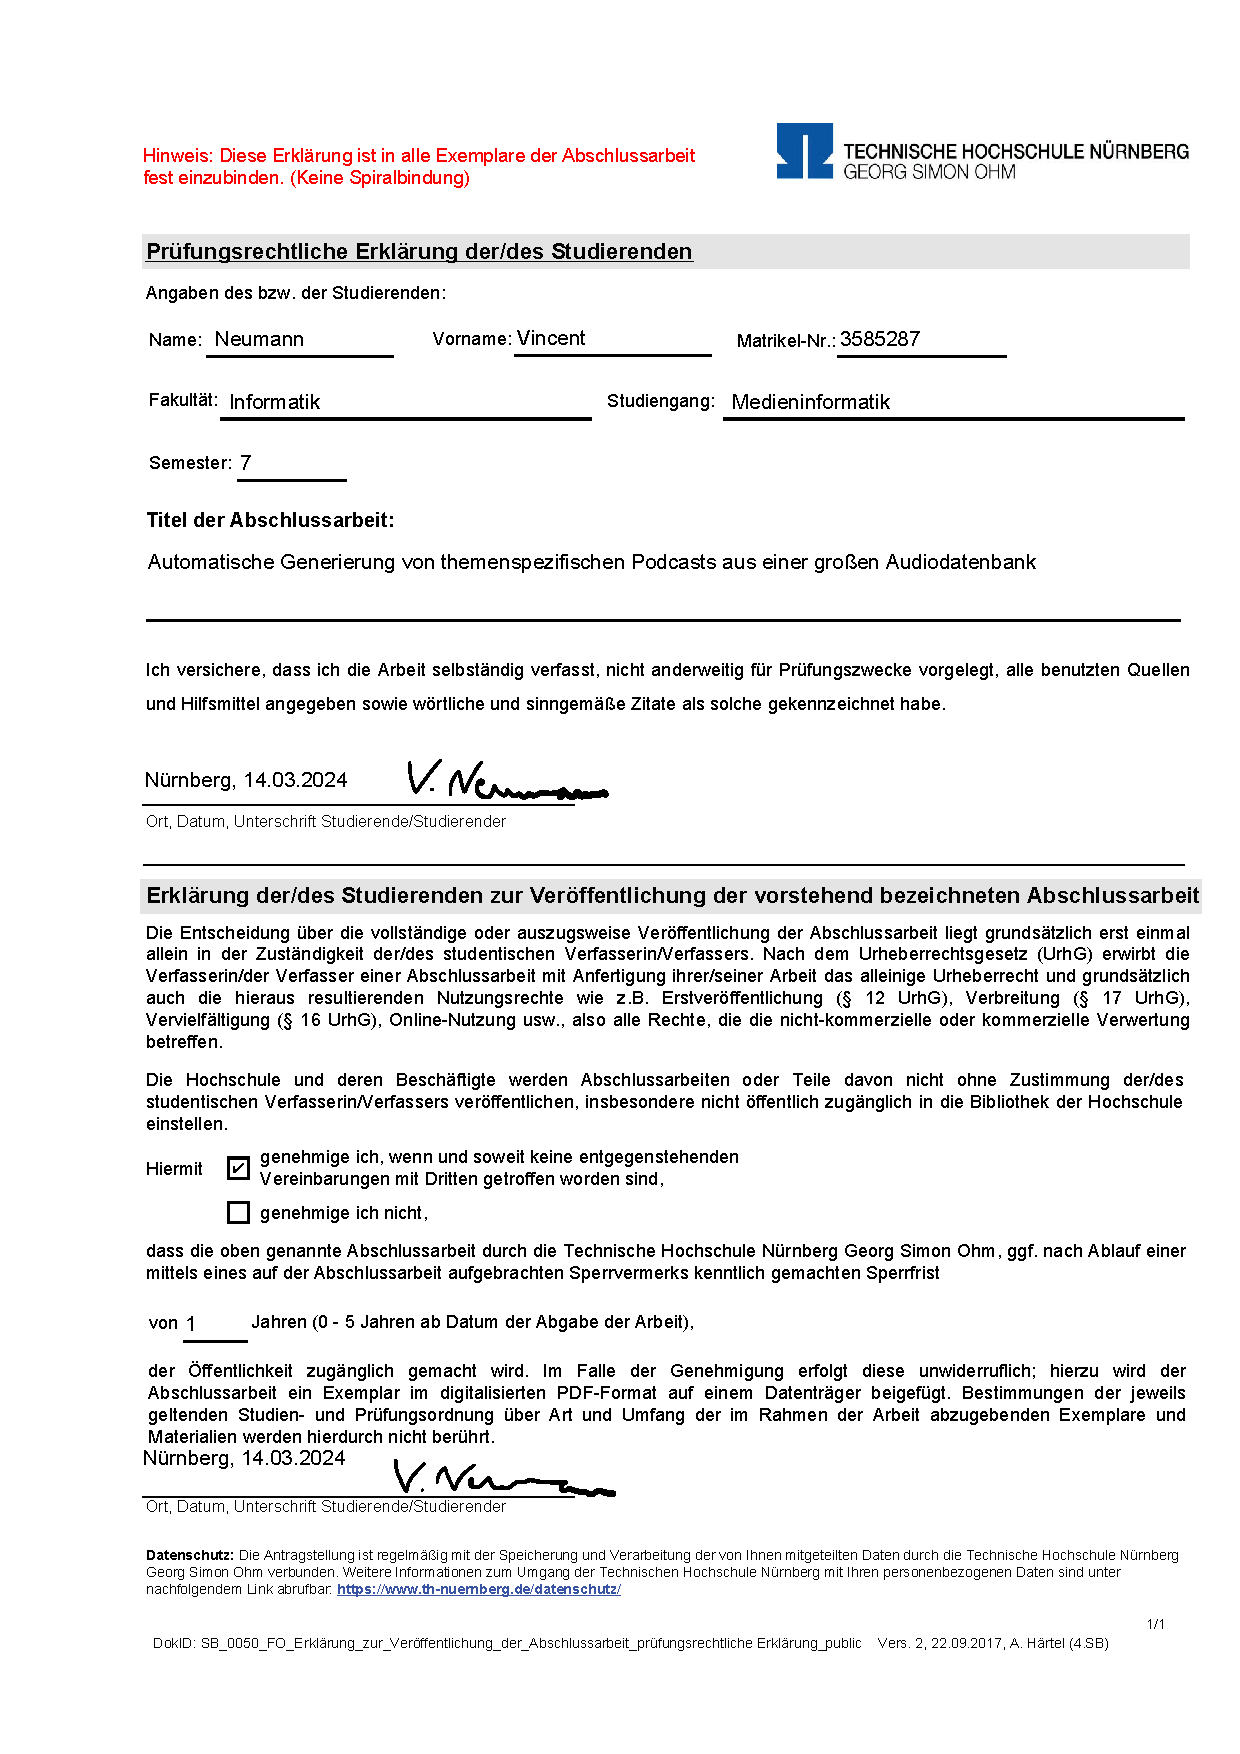
\includepdf{Pruefungsrechtliche_Erklaerung.pdf}\cleardoublepage

\thispagestyle{empty}
\section*{Kurzdarstellung}
\label{sec:kurzdarstellung}

In dieser Arbeit wird ein Ansatz für die automatische Erstellung einer Podcastepisode aus vorhandenem Audiomaterial vorgestellt. 
Dafür wird ein umfangreiches System aus mehreren Microservices erstellt, das den kompletten Verlauf von der Beschaffung der Audiodaten bis zur Bereitstellung einer Podcastepisode in einem User-Interface abdeckt.






\cleardoublepage

\tableofcontents

\mainmatter
\pagenumbering{arabic}
\chapter{Einleitung}\label{ch:intro}

\section{Motivation}

Podcasts sind für viele Menschen ein wichtiges Medium, um sich die Zeit zu vertreiben und sich über verschiedene Themen zu informieren. 
In Deutschland hören ca. 29\% der Menschen regelmäßig Podcasts \cite{newman2022}.
Dabei liegt die Nutzung der ARD-Audiothek mit 12\% auf Platz drei hinter Spotify und Youtube[TODO Quelle].
Wie Studien gezeigt haben, verbessert sich das Audioerlebnis der Zuhörer*innen dabei, wenn mehrere verschiedene Sprecher*innen dabei vorkommen \cite{kang2012}. 
Einige Podcasts werden zum Beispiel nur von einer einzigen Person vorgetragen.
Außerdem steigert das Vorhandensein verschiedener Meinungen auch das Interesse des Zuhörers an einem bestimmten Thema \cite{phillips2014}.
Neben diesen Vorteilen, ist es für die Zuhörer*innen einer Podcast Episode auch ein besonderer Aspekt der Selbstbestimmung, wenn sie die Länge einer Podcast Episode selbst festlegen können.
In dieser Arbeit wird es darum gehen, wie man diese Vorteile einer personalisierten Podcast Episode ausnutzen kann.


\section{Zielsetzung}


Das Ziel dieser Bachelorarbeit besteht darin zu untersuchen, wie sich aus umfangreichem Audiomaterial aus Radioprogrammen oder Podcasts on-the-fly ein eigener Podcast zusammenstellen lässt, der relevante Ausschnitte aus einer Vielzahl von Audiomaterial enthält.

Ein möglicher Anwendungsfall wäre ein/e Benutzer*in, die/der sich über das Thema "Überfischung der Meere" informieren möchte und dafür genau 20 Minuten während einer Autofahrt einplant. 
Das System erstellt nun einen Zusammenschnitt aus verschiedenen Podcast Episoden zu diesem Thema, der 20 Minuten lang ist und stellt ihn dem/der Benutzer*in zur Verfügung. 
Der Vorteil für den/die Nutzer*in liegt darin, dass er/sie selbst das Thema auswählen und die exakte Länge festlegen kann, um beispielsweise während einer 20-minütigen Autofahrt einen Podcast anzuhören. 
Außerdem werden das Thema von verschiednen Personen aus unterschiedlichen Blcikpunkten erklärt. 

Für die Interaktion mit dem Benutzer soll außerdem eine Grafische Benutzeroberfläche bereitgestellt werden, die dem Nutzer die Auswahl eines Themas und die Länge der Podcast  Episode ermöglicht.

\section{Überblick}

Im zweiten Kapitel werden theoretische Grundlagen zum Verständnis der später aufgeführten Technologien erklärt.

Im dritten Kapitel wird es um die Beschaffung der Datengrundlage gehen. Als Datenquelle werden Podcast Episoden aus der Audiothek der ARD benutzt. 
Dann werden verschiedene Methoden zur Transkription dieser Audiodaten beschrieben und begründet, welche Wahl der Transkription für diese Arbeit verwendet wird.

Im vierten Kapitel wird die Architektur des Systems dargestellt. 
Dabei wird besonders auf die semantische analyse der Transkriptionen eingegangen und verschiedene Aspekte des Natural Language Processing und der Large Language Models vorgestellt.

Im fünften Kapitel werden verschiedene Methoden zur semantischen Analyse evaluiert.
Dabei werden auch die verwendeten Modelle die Wahl der Anzahl und Länge der Abschnitte und die finale Zusammensetzung dieser Abschnitte erklärungt und begründet.

Im sechsten Kapitel wird ein Ausblick auf zukünftige Verbesserungen gegeben.

Im siebten Kapitel wird eine Zusammenfassung der erzielten Ergebnisse gegeben.

\chapter{Verwandte Literatur}\label{ch:related_work}

Im Bereich der automatisierten Podcasterstellung gibt es einige Versuche mittels künstlich generierter Texte und Stimmen einen eigenen Podcast zu erstellen.

In dem Artikel \qt{NewsPod: Automatic and Interactive News Podcasts}~\cite{laban2022} wird ein neuer Ansatz für die automatische Erstellung von Podcast-Episoden vorgestellt. 
Dazu wird ein interaktiver Sprachbot entwickelt, der zu bestimmten Nachrichten Fragen beantworten kann und mithilfe einer synthetisch generierten Stimme mit den nutzenden Personen interagiert.
Mehrere Machine Learning Systeme ermitteln den Inhalt von bestimmten Nachrichtenseiten und extrahieren daraus Fragestellungen, die den Inhalt des Textes widerspiegeln sollen. 
Die Autoren benutzen ein GPT-2 Sprachmodell, das auf Fragengenerierung trainiert wurde, um aus jedem Absatz 7 Fragen zu ermitteln. 
Ein weiteres Question-Answering Sprachmodell wird dann trainiert, um die Ausschnitte in den Artikeln zu finden, welche diese Fragen beantworten.  
Der Retrieval Step wird hier also nicht durch Embeddings, sondern durch ein Sprachmodell vollzogen.

Der wichtigste Aspekt dieses Artikels ist, dass die Anwendenden interaktiv mit der Software agieren und selbstgewählte Fragen mithilfe eines Mikrofons oder einer Tastatur stellen können.
Das Question-Answering Sprachmodell versucht dafür relevante Segmente aus mehreren Nachrichtenartikeln zu finden, die die Fragen der nutzenden Person beantworten.
Diese werden dann mithilfe einer synthetisch generierten Stimme von Googles Text-To-Speech API vorgelesen.

Die Autoren dieses Papers führten außerdem zwei Studien zur Nutzung dieses Systems durch.
Der Gegenstand der ersten Studie ist, inwieweit die Zufriedenheit einer Testgruppe mit der Erzählweise des Textes und der automatisch generierten Stimme des Sprechers korreliert. 
Darin konnten die Autoren feststellen, dass einer ihrer Ansätze, QA Best, so erfolgreich war, dass 80\% der Testpersonen angaben, dass sie dieses System in Zukunft nutzen würden, um Nachrichten zu konsumieren.
Die zweite Studie untersucht die Interaktion der Zuhörenden während der Benutzung des Systems. 
Diese Studie kam zu dem Schluss, dass zwar die Bereitschaft eigene Fragen zu stellen mit 85\% der Zuhörenden sehr hoch war, die Zufriedenheit der Testenden mit der Qualität der Antworten aber sehr gering ausfiel, da 76\% der Antworten als verwirrend eingestuft wurden.~\cite{laban2022}


In einem weiteren für diese Arbeit relevanten Paper~\cite{jones2021} werden die Ergebnisse der Text Retrieval Conference (TREC) 2020 für die Podcastanalyse vorgestellt.
Für diese Aufgabe analysierten die Teilnehmer einen großen Datenbestand an Podcasttranskripten.
Die Teilnehmer versuchten aus über 100.000 Podcasttranskripten die wichtigsten Segmente zu verschiedenen Themen herauszufiltern.
Im Vorfeld wurden die Transkripte durch ein System zur Automatic Speech Recognition (ASR) erstellt.
Jedes Transkriptsegment ist dabei jeweils genau zwei Minuten lang und überlappt sich um eine Minute mit einem folgenden Segment.
Die entsprechenden Aufgabenstellungen sind in drei Kategorien eingeteilt: \qt{topical}, \qt{re-finding} und \qt{known items}.
Bei der Kategorie \qt{topical} wird verlangt, passende Segmente zu einem bestimmten Thema zu finden.
Beim \qt{re-finding} geht es darum, einen zuvor bekannten Audioinhalt wiederzufinden.
Dabei waren nur Teile des Audioinhaltes oder bestimmte Rahmenbedingungen vorgegeben (z.B. eine Podcast-Episode, welche die Person vor einer Woche hörte).
In der letzten Kategorie den \qt{known items} sind bereits der Titel bzw.\ weitere Metainformationen bekannt.
Die einzelnen Themen verfügten dabei außerdem noch über eine Beschreibung, die spezifiziert, was eine Testperson von der Suche mit diesem Prompt erwarten würde.


Insgesamt nahmen neun Teilnehmer an dieser Aufgabe teil und reichten eine Lösung ein.
Darunter Universitäten aus den USA und Dublin sowie ein Team des Musikstreaminganbieters Spotify.
Die Evaluation der Ergebnisse wurde manuell durchgeführt.
Verschiedene Gutachter des TREC bewerteten die Ergebnisse der Teilnehmer auf einer Skala von 5 (perfekt) bis 0 (nicht passend).
Am besten schnitten dabei die Lösungen der Universität Maryland ab, die zur Datenaufbereitung eine Mischung aus Stemming und Word2Vec benutzten und für die Retrievalfunktion die Search Engine Indri einsetzten.
Die Indri Search Engine wurde von der University of Massachusetts und Carnegie Mellon University aufgebaut, wird aber zurzeit nicht mehr weiterentwickelt~\cite{lemur}.


Speziell für deutsche Audioinhalte ist ein Artikel zu erwähnen, indem das Fraunhofer-Institut für Intelligente Anlyse- und Informationssysteme (IAIS) 2015 die Audiominig Plattform medas vorstellt~\cite{maroni2020}.
Diese soll für die ARD-Audiothek die Suchfunktionen für verschiedene Audioinhalte verbessern.
Dazu erstellten die Forscher ein System, dass diese Inhalte automatisch mit ASR transkribieren, eine Spracherkennung durchführen und Keywörter extrahieren kann.
Diese Daten sind über eine REST Schnittstelle abrufbar.
Allerdings sind viele der beschriebenen Technologien mittlerweile nicht mehr State-of-the-Art und spielen deswegen in dieser Arbeit kaum eine Rolle.~\cite{maroni2020}
In \autoref{ch:method} wird darauf näher eingegangen.

\chapter{Ausgangslage und theoretische Grundlagen}\label{ch:theoretical}


\section{Information Retrieval}

Das Ziel dieser Arbeit besteht darin, eine Schnittstelle für einen Hörenden zu erstellen, die ihm ermöglicht, einen Zusammenschnitt aus vielen verschiedenen Podcast Episoden zu erstellen, der genau zu einem Thema passt. 
Die wichtigste Aufgabe besteht also darin, die wesentlichen Abschnitte aus den Episoden herauszufinden. 
Dazu muss das System verstehen, welche Abschnitte zu verschiedenen Anfragen passen. 

Das Thema Information Retrieval (Informationsrückgewinnung) bezeichnet den Vorgang, aus einer großen Menge unsortierter Daten bestimmte Informationen wieder zu extrahieren.
Im Gegensatz zu Data-Mining werden dabei keine neuen Daten erschaffen, sondern lediglich bereits existierendes Wissen wieder zur Verfügung gestellt.
Ein bekanntes Beispiel eines Information Retrieval Algorithmus ist der PageRank Algorithmus für die Suchmaschine Google.
Suchmaschinen sind das Musterbeispiel eines Information Retrieval Systems.
Ein User gibt Stichworte ein, über die er mehr Informationen erhalten möchte und erhält daraufhin Links zu Webseiten, die diese Informationen wahrscheinlich enthalten.

In dieser Arbeit wird die Informationsrückgewinnung auf Basis der Daten von Podcasttranskripten betrieben.
Dazu werden die Techniken der Text Embeddings benutzt, um relevante Informationen zu einem bestimmten Thema aus einer großen Anzahl an Dokumenten zurückzugewinnen.



\section{Embeddings}

\subsection{Embeddings als Computersprache}

Text Embeddings sind ein Weg die menschliche Sprache für Computer verständlich zu machen. 
Die menschliche Sprache ist ein hochkomplexes Konstrukt mit einer Grammatik, die sehr viel flexibler, kreativer, vieldeutiger und komplexer ist als Maschinensprache. 
Es gibt viele kleine Bedeutungsnuancen, diese Sprache ist stark von dem allgemeinen Wissensstand der Welt geprägt und sie ändert sich im Laufe der Zeit. 
Das alles macht es für Computer sehr schwierig die menschliche Sprache zu verstehen. 
Neuere Forschung im Bereich des Natural Language Processing bietet einige Ansätze, um dieses Problem zu lösen. 
Es gibt dazu viele verschiedene Methoden, die alle darauf abzielen, Worte oder Texte in Vektoren umzuwandeln, die den Inhalt dieser Worte oder dieser Texte repräsentieren.
Diese Vektoren nennt man Embeddings.
Das Ziel dieser Embeddings besteht für unseren Zweck darin, eine Suchfunktion zu beschreiben, die auf eine Anfrage (Query) hin, passende Dokumente aus einem großen Korpus an Dokumenten liefern kann.

\subsection{Tokenisierer}

Um Textsequenzen mithilfe von Embeddings zu verarbeiten, werden diese Texte zunächst in Tokens zerlegt, bevor sie von einem Embeddingmodel embedded werden.  
Ein Token kann dabei je nach Modell ein einziges Wort, mehrere Worte oder nur ein Bruchteil eines Wortes sein.
In Machine Leerning Anwendungen nutzt man dafür verschiedene Tokenisierer.
Es gibt einfache Tokenisierer, wie Whitespace Tokenisierer, die einen Text einfach an Leerzeichen teilen und die einzelnen Wörter als Tokens behandeln.
Etwas besser sind Wort Tokenizer, die auch Satzzeichen erkennen und dadurch Punkte und Kommata nicht an das Ende des vorangegangenen Wortes anhängen. 
Einen solchen Tokenizer nutzt beispielsweise spaCy, um "Linguistic Features" zu bestimmen \cite{honnibal2017}.
Es gibt Subword tokenisierer, die Worte nocheinmal in kleinere Abschnitte teilen.
Das Byte-Pair Encoding versucht aufgrund von statistischen Methoden, häufig vorkommende zusammenhängende Zeichenfolgen als Tokens zu identifizieren.
Diese Art Tokenizer wird am öfftesten für die Eingabe bei Transformern genutzt \cite{zouhar2023}.
Die Transformermodelle von OpenAI benutzen beispielsweise tiktoken als Tokenizer \cite{tiktoken2024}, das BERT Modell von Google benutzt den WordPiece Tokenizer.

\subsection{Geschichte der Embeddingverfahren}

Die ersten Algorithmen mit dem Ziel, eine große Anzahl von Dokumenten durchsuchen zu können, waren Suchalgorithmen wie TD-IDF oder BM25, die in den 1970er Jahren aufkamen.
Diese versuchten Worthäufigkeiten als Anhaltspunkt zu nehmen, um Ähnlichkeiten zwischen Dokumenten zu erkennen und Suchfunktionen aufzubauen. 

Semantische Analysen begannen erst ab ca. 1990 mit der Latenten Semantischen Analyse (LSA).
Diese verwendet Eigenvektoren, um aus einer Term-Frequency Matrix versteckte (latente) Eigenschaften zu ermitteln, welche die Dokumente besser repräsentieren als die TF Matrix an sich. 
Es werden von diesen Eigenvektoren nur die wichtigsten ausgewählt, sodass jedes Dokument sehr gut als eine Linearkombination dieser Vektoren repräsentiert werden kann.
So werden nur noch die Koeffizienten dieser Vektoren gespeichert und man kann von einer Dimensionsreduktion profitieren.
Die resultierenden Koeffizienten-Vektoren sind nun nicht mehr spärlich besetzt sondern dicht und die resultierenden Eigenvektoren bilden häufig latente Themen der Dokumente ab.

Wirkliche semantische Word Embeddings erlangten erst mit der Veröffentlichung von Word2Vec (2013) eine breitere Nutzung. 
Word2Vec verwendet ein neuronales Netz, um mithilfe der benachbarten Wörter Kontextinformationen über das eigentliche Wort zu erhalten. 
Dafür gibt es die beiden Ansätze Continuous Bag of Words und Skip-Gram.
Bei dem Ansatz Continuous Bag of Words erhält das Neuronale Netz die umgebenden Wörter als Input und das Model hat die Aufgabe daraus das Zielwort zu ermitteln. 
Dieses Verfahren wird in einem Sliding Window für jedes Wort aus einem Text wiederholt. 
Für einen bestimmten Korpus aus verschiedenen Dokumenten kann dieses Modell dadurch die Beziehungen verschiedener Wörter zueinander und die Ähnlichkeit verschiedener Wörter, die oft in gleichem Kontext vorkommen, erlernen. 
Das Verfahren des Skip-Gram funktioniert ähnlich, allerdings wird dabei für jedes Wort versucht, die umliegenden Wörter zu ermitteln. 
Dieser Ansatz dauert länger im Training, hat aber den Vorteil, dass er auch seltener vorkommende Wörter gut repräsentieren kann.

Ein Jahr später wurde GloVe (Global Vectors for Word Representations) als Forschungsprojekt von der Stanford Universität vorgestellt.
GloVe verbindet Konzepte aus LSA und Word2Vec, indem es auf der Faktorisierung einer globalen Matrix beruht, aber die Distanz von Wörtern zueinander mitberücksichtigt.
Dadurch schaffte GloVe eine weitere Verbesserung der Embeddings und wird heutzutage noch unter anderem in NLP Bibliotheken wie spaCy verwendet.[englische Wikipedia referiert auf Buch aus 2018]

Im Jahre 2018 wurde der Ansatz ELMo (Embeddings from Language Model) für Word Embeddings vorgestellt.
Dieser benutzt bidirektionale Long Short Term Memory Modelle (LSTM), um daraus Embeddings zu generieren.
LSTM Modelle basieren auf Rekurrenten Neuronalen Netzen (RNN) und gehören zu den Sequenz to Sequenz Modellen. 
Sie bestehen dabei aus einem Encoder und einem Decoder.
Der Encoder codiert eine Inputsequenz, zum Beispiel ein Dokument, zu einem Embeddingvektor. 
Der Decoder dekodiert diesen Embeddingvektor wieder in eine Sequenz, z.B. eine Zusammenfassung des Dokuments. [Quelle]
Für ELMo ist dabei nur der Encoder Teil wichtig.
Dabei werden zwei Layer von Forward und Backward LSTMs eingesetzt, die für jedes Wort den Kontext vor und nach dem Wort berücksichtigen, um semantische Embeddings zu erstellen. [Quellen]

Ein halbes Jahr später wurden die Erstellung von Word und Sentence Embeddings durch BERT revolutioniert.
BERT (Bidirectional Encoder Representations from Transformers) \cite{devlin2019} ist ein auf NLP Aufgaben spezialisierter Transformer.
Das Modell wurde von Google 2019 entwickelt und war seinerzeit das beste Modell, da es in elf verschiedenen Aufgaben im Bereich des NLP State-of-the-art Ergebnisse lieferte.
Es ist auf zwei Datenbeständen, dem BooksCorpus mit 800 Millionen Wörtern und der englischen Wikipedia mit 2,5 Milliarden Wörtern trainiert worden. 
Die Aufgaben im Trainierprozess waren die Next Sentence Prediction (NSP), bei der das Modell entscheiden muss, ob zwei Sätze wahrscheinlich zusammen vorkommen und das Masked Language Modeling, bei der das Modell unkenntlich gemachte Wörter in Sätzen wiederherstellen soll.
Dadurch hat BERT sowohl auf Wortebene als auch auf Satzebene wichtige Merkmale der Sprache gelernt.
Durch die große Auswahl an verschiedenen Themen im Trainingsprozess kann das Model für viele verschiedene Sachverhalte sinnvolle semantische Embeddingvektoren erstellen.
\cite{devlin2019}


Seit der Entdeckung der Transformerarchitektur und der Entstehung von BERT entwickelt sich der Bereich der Embeddingmodelle rasant.
Täglich werden neue Modelle publiziert und im Abstand von wenigen Wochen erreichen neue Modelle State-of-the-art Performance auf populären Benchmarks wie MTEB.  


\subsection{Embeddingvektoren}

\subsubsection{Dünne Vektoren}

Embeddings können in zwei verschiedene Kategorien eingeteilt werden: dünne Vektoren und dichte Vektoren.

Dünne Vektoren, wie der TF-IDF Algorithmus und der BM25 Algorithmus, versuchen syntaktische Eigenschaften von Dokumenten zu erfassen.
Term Frequency - inverse Dokument Frequency (TF-IDF) ist ein Algorithmus, der es erlaubt, Dokumente nach Keywörtern zu durchsuchen.
Das Verfahren verwendet Worthäufigkeiten (Term-Frequency), um Dokumente, in denen ein Wort häufiger vorkommt zu bevorzugen.
Außerdem verwendet es die generelle Auftrittsrate von Wörtern (Inverse Document Frequency) um Wörtern, die seltener vorkommen, mehr Gewicht bei der Suche einzuräumen.

Daraus bildet der TF-IDF Algorithmus einen dünnbesetzten Vektor, der die Anzahl und Seltenheit jedes im Dokument vorkommenden Wortes abbildet. 
Dünnbesetzt heißt in diesem Zusammenhang, dass der Vektor viele Einträge mit dem Wert 0 besitzt. 
Das folgt aus der Bedingung, dass diese Vektoren untereinander vergleichbar sein müssen und dadurch Einträge für jedes Wort besitzen, welches im gesamten Korpus an Dokumenten vorkommt.
Jedes einzelne Dokument enthält dabei aber nur einen Bruchteil der Gesamtwörter und damit viele Nullwerte.

Best Matching 25 (BM25) ist eine Familie von Algorithmen die versuchen, den TF-IDF Algorithmus zu verbessern, indem sie die Priorisierung langer Dokumente und zu oft vorkommende Worte ausgleichen.

Außerdem kann man diese Algorithmen noch anpassen, sodass sie auch N-Gramme als Einträge der Vektoren miteinbeziehen. 
Das heißt, dass nicht nur einzelne Wörter berücksichtigt werden, sondern auch häufig zusammen vorkommende Wörter (N-Gramme) als einzelnes Token in dem Vektor abgebildet werden. 
Das bewirkt zwar, dass die Ähnlichkeit der Dokumente in der Regel besser ermittelt werden kann, vergrößert aber die Vektoren.

\subsubsection{Dichte Vektoren}

Ein relativ moderner Ansatz besteht in der Suche mithilfe von dichten Embedding Vektoren. 
Dabei wird versucht, die Semantik (also die Bedeutung) der einzelnen Segmente mathematisch mithilfe eines Vektors zu repräsentieren. 
Dieser Vektor soll dann zur Suche nach Ähnlichkeit eingesetzt werden. 
Ein Vektor, der aus dem Satz „Ich sitze auf einer Bank im Grünen“ besteht und ein Vektor mit dem Satz „Im Park steht eine alte Bank“ sollen dabei sehr ähnlich zueinander sein. 
Der Embeddingvektor des Satzes „Ich gehe in die Bank und hebe Geld ab“ aber sollte dazu wenig Ähnlichkeit aufweisen. 
Hierbei soll erkannt werden, dass sich die ersten beiden Sätze auf eine Bank zum Sitzen in der Natur beziehen und der dritte Satz ein Geldinstitut betrifft. 
Ein solch filigranes Verständnis der Bedeutung ist nicht einfach zu erreichen. 
Ein stochastischer Algorithmus würde die Unterschiede bei solchen Homonymen in den meisten Fällen nicht erkennen können. 
Stochastische Algorithmen wie z.B. TF-IDF haben auch Probleme mit Negierungen, wie zum Beispiel in „Ich habe nichts gegessen.“ und „Nichts habe ich heute gemacht außer gegessen“.

Für unsere Aufgabe ist es sinnvoll, nicht nur inhaltliche Vergleiche zu erstellen, die überprüfen, ob zwei Sätze ungefähr die gleiche Bedeutung haben, wie "Die Sonne bringt mich zum schwitzen" oder "Ich schmelze in der Hitze".
Besser wäre eine asymmetrische Ähnlichkeit, wie sie bei Frage und Antwortpaaren vorkommt.
Zum Beispiel wäre auf die Frage: "Welche Farbe hat der Himmel bei Sonnenuntergang?" ein gute Antwort: "Der Himmel hat bei Sonnenuntergang oft orange und rosa Farbtöne."  und nicht der Satz "Wie sieht der Himmel am Abend aus?"
Diese asymmetrische Ähnlichkeit ist schwerer zu ermitteln, da man normalerweise in der Antwort Informationen findet, die in der Frage nicht vorkommen.

\subsubsection{Dimensionalität von Embeddingvektoren}

Die Dimensionalität von verschiedenen Embeddings hat Einfluss auf deren Performance.
Kleinere Embeddings verbrauchen weniger Speicherplatz und lassen sich schneller untereinander vergleichen, was den Retrieval Prozess beschleunigt.
Andererseits bietet eine kleinere Dimensionalität auch weniger Möglichkeiten für die LLMs, semantische Informationen darin zu speichern.
Das heißt aber nicht, das größere Embeddingvektoren auch gleichzeitig die Semantik besser repräsentieren müssen.
Dies hängt vor allem damit zusammen, wie leistungsstark die Architektur des Modells ist und wie viele und welche Trainingsdaten zum trainieren verwendet wurden.
Das Modell "voyage-lite-02-instruct" belegt zum Beispiel auf dem Massive Text Embedding Benchmark Leaderbord mit einer Dimensionalität von 1024 den Platz 2.
Auf den Plätzen 3-5 liegen aber Embeddingmodelle mit einer Dimensionalität von 4096.


\subsection{Ähnlichkeitsvergleiche}

Mithilfe der Embedding Vektoren können wir Sätze finden, die zueinander Ähnlich sind. 
Aber was bedeutet überhaupt ähnlich? 
Die Vektoren des BERT Models sind 768 Dimensional, haben also 768 Gleitkommazahlen gespeichert, die zwischen -1 und 1 liegen. 
Diese Gleitkommazahlen Vektoren könnte man auch als Feature Vektoren begreifen. 
Zum Beispiel könnte die erste Zahl dieses Vektors für die Erwähnung von Professoren in dem Satz stehen (-1 für keine Professoren; 1 für viele Professoren). 
Die zweite Zahl könnte für das Thema Essen stehen (-1 für wenig mit Essen zu tun; 1 für sehr viel mit Essen zu tun). 
Damit hätte der Satz „In der Mensa gibt es jeden Tag Currywurst mit Pommes“ an der ersten Stelle vielleicht eine 0,1, weil der Begriff „Mensa“ leicht mit Uni und Professoren konnotiert wird und die zweite Stelle würde bei 0,94 liegen, da es in dem Satz offensichtlich um das Essen handelt. 
In der Realität wird das Model sehr wahrscheinlich nicht so für Menschen offensichtlichen Merkmale lernen. Ein Grund dafür ist, dass das Model vor allem pro Eintrag eine linearkombination von verschiedenen Menschenoffensichtlichen Merkmalen lernen wird, also jede Zahl eine überlagerung verschiedener Eigenschaften darstellt. 
Eine forschungsrichtung, die versucht solche Modelausgaben Menschenlesbar zu gestalten liegt in der Explainable AI \cite{hassija2024}.

Um die Ähnlichkeit von diesem Satz zu der Frage „“ zu bestimmen nutzen wir die Cosinus distanz als Maß. 
Es gibt auch die Euclidische Distanz, allerdings gestaltet sich dabei das Problem der Vector Normalisierung.


Diese Komplexen semantischen Unterschiede, oder Gemeinsamkeiten zu erkennen erfordert etwas mehr Raffinesse.

Andere Distanzmaßen:
Manhatten Distanz (nur x oder y Achse)
Hamming Distanz (Anzahl verschiedener Einträge)

\subsubsection{Euklidische Distanz}

Die Euklidische Distanz von zwei Vektoren kann man über den Satz des Pythagoras berechnen.
Dafür nimmt man für jede Dimension die Differenz beider Vektoren in dieser Dimension, quadriert diese und summiert alle Quadrate zusammen, um dann die quadratwurzel darüber zu ziehen.
Für die beiden Vektoren 
$\begin{pmatrix}0\\1\end{pmatrix}$
und 
$\begin{pmatrix}-1\\0\end{pmatrix}$
wäre die

Euklidische Distanz $\frac{1}{\sqrt{2}}$, da $\sqrt{(0-(-1))^2 + (1-0)^2}=\frac{1}{\sqrt{2}}$

Dieses Distanzmaß ist sensibel gegenüber der Länge der Vektoren.
Wenn die Vektoren nicht normiert wurden, kann die Euklidische Distanz sehr groß werden und die Ergebnisse einer Ähnlichkeitssuche verfälschen.


\subsubsection{Cosinus Distanz}

Ein weiteres Ähnlichkeitsmaß kann man über den Winkel zwischen zwei Vektoren definieren.
Dieser Winkel ist unanhängig davon, wie lang die Vektoren sind, immer gleich.
Die weitverbreiteste Methode um diesen Winkel zu messen, ist über die Cosinus Ähnlichkeit.
Diese berechnet den Cosinus des Winkels und kann einfach über die Formel

$\text{cosine\_similarity}(\mathbf{a}, \mathbf{b}) = \frac{\mathbf{a} \cdot \mathbf{b}}{\|\mathbf{a}\| \|\mathbf{b}\|}$

berechnet werden.
Dabei wird für beide Vektoren zunächst das Skalarprodukt bestimmt.
Das Skalarprodukt besitzt die Eigenschaft groß zu sein, wenn beide Vektoren in ähnliche Richtungen zeigen und kleiner, wenn beide Vektoren in unterschiedliche Richtungen zeigen.
Dabei hat die Länge der unterschiedlichen Vektoren einen Einfluss auf die Größe des Skalarproduktes.
Um dieser Verzerrung entgegenzuwirken, wird das Skalarprodukt durch das Produkt der Beträge der Vektoren geteilt.
Dadurch erhält man den cosinus des Winkels zwischen diesen beiden Vektoren.

Wenn beide Vektoren vorher normiert wurden, das heißt der Betrag der Vektoren gleich Eins ist, ist die Cosinus Distanz gleich der Skalarprodukt Distanz der beiden Vektoren.
Außerdem kann in diesem Fall die Euklidische Distanz asu der Cosinus Distanz errechnet werden durch die Formel: 

$\text{Euclidean distance} = \sqrt{2 - 2 \cos(\theta)}$

\section{Transformer Architektur}

\subsection{Sequenz to Sequenz Modelle}

Eine Transformerarchitektur ist eine der modernsten und leistungsfähigsten Architekturen, um eine Vielzahl von  NLP Aufgaben zu lösen. 
Sie bildet dabei den Nachfolger bzw. Konkurrenten zu den bis dato vorherrschenden Rekurrenten neuronalen Netzen (RNN), Gated Recurrenten Units (GRU) oder Long-Short Term Memory Systems (LSTM). 
Ähnlich zu diesen Architekturen ist auch der Transformer ein Sequenz-zu-Sequenz-Modell. 
Der Encoderteil nimmt als Eingabe eine Folge von Tokens (einen Satz, eine Audiodatei) und der Decoderteil bildet daraus eine andere Sequenz (einen Satz, eine Audiodatei). 
% In diesem Abschnitt gehen wir nur auf den Encoder ein, weil er die Embeddings erstellt.

Der Unterschied von Sequenz-zu-Sequenz-Modellen zu einem gewöhnlichen feedforward neuronalen Netz besteht darin, dass die Eingabe- und Ausgabesignale auch Sequenzen mit variabler Länge sein können.
Gewöhnliche künstliche neuronale Netze haben eine feste Anzahl an Eingangs- und Ausgangsneuronen, was es ihnen nur erlaubt, Aufgaben zu lösen, bei denen die Eingangs- und Ausgangsdaten eine bestimmte Länge aufweisen.
Anwendungsfälle für künstliche neuronale Netze sind zum Beispiel Frühwarnsysteme oder Klassifikationsaufgaben (z.B. Ziffererkennung).

\subsection{RNNs, LSTMs und GRUs}

Rekurrente neuronale Netze (RNNs) stellen eine Weiterentwicklung von feedforward neuronalen Netzen dar, indem sie eine Rückkoppelung des Ausgabesignals erlauben und somit eine variable Länge an Eingabesignalen verarbeiten können.
Das Eingabesignal muss einer Sequenz entsprechen und wird dafür in Tokens zerlegt.
Jedes Token wird dabei einmal durch das RNN propagiert bis ein Ausgabeembedding für dieses Token produziert wurde.
Das Ausgabeembedding aus der vorherigen Iteration wird dann zusammen mit dem nächsten Token in der Sequenz als Eingabe für die nächste Iteration verwendet.
Dadurch wird die gesamte Sequenz nacheinander in diesem Netz verarbeitet, wobei jedes Token den Kontext der vorherigen Tokens als Embedding mitgeliefert bekommt.
Am Ende liefert ein RNN dann ein einziges Embedding, welches die gesamten Informationen der Sequenz repräsentieren soll.

Ein Problem, welches diese Architekturen besitzen, ist das Problem des Vanishing Gradient.
RNNs versuchen immer im Encoder die gesamte Inputsequenz von links nach rechts (forward) oder von rechts nach links (backward) zu verarbeiten, um daraus ein einzelnes Embedding zu erstellen.
Informationen, die in der Mitte der Sequenz vorkommen, werden wahrscheinlich von danach folgenden Informationen überschrieben, weil das Modell versucht, alle Informationen in derselben Matrix zu speichern. 

Die Ansätze des Long-Short Term Memory System (LSTM) und der Gated Recurrenten Unit (GRU) versuchen dieses Problem zu lösen, indem sie Gates einsetzen.
Diese Gates bestimmen, welche Informationen aus dem vorherigen Embedding durch das Embedding der nächsten Iteration überschrieben werden dürfen.
Dadurch können sie wichtige Informationen länger speichern.
Bei einem LSTM werden dafür drei verschiedene Gates benutzt: das Forget Gate, das Input Gate und das Output Gate.
Jedes dieser Gates hat wiederum eine bestimmte Anzahl an Parametern, die bestimmen welche Informationen vergessen, welche für den Input der nächsten Iteration benutzt und welche bei der nächsten Iteration ausgegeben werden.
Alle diese Parameter müssen beim Training des LSTMs mittrainiert werden, was zu einem komplizierten Model und zu einem langsamen Trainingsprozess führt.
Bei GRUs gibt es nur ein Gate: das Update Gate.
Sie haben dadurch weniger Parameter, die trainiert werden müssen und vereinfachen damit den Trainingsprozess.
\cite{pirani2022}

\subsection{Transformer Encoder}

Der größte Unterschied der Transformerarchitektur zu RNNs, GRUs und LSTMs ist der Attention Mechanismus.
RNNs, GRUs und LSTMs sind darauf angewiesen, den Input sequentiell Token für Token zu verarbeiten, da jede Zelle als Input das Embedding der vorausgehenden Zelle benötigt.
Das macht das Training eines Models sehr zeitaufwendig.

Der große Vorteil der Transformer ist, dass sie parallelisierbar sind.
Alle Tokens einer Inputsequenz können synchron verarbeitet werden. 
Dabei wird für jedes Token zunächst durch ein vorher ermitteltes Word Embedding ersetzt.
Der Mechanismus des Positional Encodings stellt sicher, dass das Modell die Reihenfolge der Token mitberücksichtigen kann.
Dieser Mechanismus berechnet aufgrund der Position des Tokens in der Sequenz ein Positional Embedding auf der Grundlage von Sinus- und Cosinusfunktionen und addiert es mit dem vorherigen Word Embedding.
Das resultierende Embedding enthält damit sowohl Informationen über das Token selbst durch das Token Embedding und über die Position in der Sequenz durch das Positional Encoding.


\subsection{Multihead Self Attention}

Transformer setzen Multihead Self Attention ein. 
Der positional encoded Input wird von mehreren self Attention Köpfen verarbeitet, der sogenannten Multihead Self Attention. 
Jeder dieser Köpfe spaltet den Input in Query, Key und Value Matrix auf, indem es die ursprüngliche Embeddingmatrix jeweils mit einer vortrainierten Query-, Key- und Valuematrix multipliziert.
Die resultierenden Matrizen werden dann mithilfe folgender Formel zur Attention Matrix umgewandelt:

$Attention(Q,K,V)=softmax(\frac{QK^t}{\sqrt{d_k}})*V$

Der Parameter d stellt dabei die Dimension der Matrix k dar.

Um die Formel besser zu verstehen, wird an einem Beispiel demonstriert, was die einzelnen Matrizen für Aufgaben besitzen.
Als Eingabe wird der Satz: "Alice fuhr gestern durch die Nürnberger Innenstadt" benutzt.
Die Query Matrix beschreibt nun eine Frage an diesen Satz, zum Beispiel "Wer?".
Wie genau diese Fragen aussehen, ist nicht leicht zu ermitteln und wird nur in seltenen Fällen so ausfallen, wie auch Menschen nach bestimmten Informationen fragen.
Wichtig ist jedoch, dass in jedem Attention Kopf eine bestimmte Frage gestellt wird.
Die Key Matrix hat nun die Antwort darauf, wo diese Informationen im Satz stehen könnten, also wahrscheinlich im ersten Wort. 
Die beiden Matrizen werden nun multipliziert, um die Position der Antwort auf die Frage zu erhalten. 
Das Ergebnis wird durch Division mit der Dimension der Matrix skaliert und anschließender Softmax-Funkion normiert, um die Relevanz der Schlüssel anzupassen.
Anschließend wird die angepasste Fragen-Schlüssel Matrix mit der Value Matrix multipliziert, welche die Informationen der Sequenz beinhaltet. 
Die resultierende Matrix würde dann die Information beinhalten, dass die Antwort auf die Frage "Wer?" für den Satz "Alice fuhr gestern durch die Nürnberger Innenstadt" wahrscheinlich "Alice" ist.

Die verschiedenen Köpfe der Multihead Self-Attention liefern nun verschiedene Antworten auf verschiedene Fragen und versuchen damit die Informationen der Sequenz zu codieren.
Im Anschluss werden die verschiedenen Matrizen konkateniert und in einem weiteren feedforward neuronalen Netz in Ihrer Dimensionalität reduziert.
Die finale Embeddingmatrix kann für verschiedene Funktionalitäten eingesetzt werden.

Die Transformerarchitektur benutzt dieses Embedding, um damit im Decoder wieder neue Tokens zu erstellen.
Dafür wird eine ähnliche Vorgehensweise wie im Encoder betrieben.
Der größte Unterschied zwischen dem Encoder und dem Decoder ist, dass der Encoder den Input nur ein einziges Mal verarbeitet und die daraus entstandene Embeddingmatrix nicht mehr neu berechnet werden muss.
Dadurch ist dieser Schritt sehr schnell.
Im Gegensatz dazu wird die Decoderphase für jedes einzelne Outputtoken neu durchlaufen.
Zunächst wird dabei wieder eine Self-Attention Matrix über den gesamten bisherigen Ausgabetokens generiert.
Die Self-Attention Matrix wird dann genutzt, um eine weitere Attention Matrix zu errechnen.
Diese benötigt nun wieder eine seperate Query-, Key- und Valuematrix.
Im Vergleich zur Self-Attention werden dabei aber nicht alle Matrizen aus derselben Embeddingmatrix errechnet.
Nur die Querymatrix wird aus der vorher generierten Self-Attention Matrix generiert.
Die Key- und die Valuematrix werden aus der Embedding Matrix des Encoders berechnet. 
Dadurch wird die Information aus dem Userprompt bei der Generierung jedes einzelnen Tokens mitberücksichtigt. 
Die resultierenden Matrizen aller Attentionköpfe werden wieder durch Feedforward Netze propagiert, um sie zusammenzuführen und die Dimensionalität anzupassen.
Am Ende wird die ganze Matrix durch eine Softmax Funktion geleitet, die dann die Ausgabewahrscheinlichkeiten für alle Token generiert.
Das heißt die Ausgabe ist ein Vektor, der als Dimensionalität die Länge des Vokabulars der Token besitzt.
Welches Token am Ende generiert wird, kann zum Beispiel mit einem Greedy-Algorithmus bestimmt werden, der immer das Wort mit der größten Wahrscheinlichkeit auswählt.
Andere Auswahlmöglichkeiten wären zum Beispiel mit einem Beam-Search Algorithmus möglich, bei dem mehrere Sequenzen generiert werden, um erst später zu schauen, welche Sequenz insgesamt die höchste Wahrscheinlichkeit besitzt.
In dieser Phase kann auch eine Zufallsvaiable eingeführt werden, die immer ein Token aus den wahrscheinlichsten Token auswählt, um bei mehrfacher Wiederholung eines Prompts verschiedene Ergebnisse zu liefern.

Um bei dem Beispiel von oben zu bleiben, würde der Decoder zum Beispiel versuchen, den Satz zu vollenden mit  "Alice fuhr gestern durch die Nürnberger Innenstadt und bewunderte die beeindruckenden mittelalterlichen Bauwerke."
\cite{vaswani2023}

\myfigure{transformer_architecture.png}{Transformer Architekut}{transformer_architecture}


\section{Large Language Model}

Large Language Model (LLM) bezeichnet ein Language Model, das auf vielen Parametern trainiert wurde. 
Dabei versteht man unter Language Model ein Sprachmodell in Anlehnung an die natürlicher Sprache.
Die meisten modernen LLMs basieren auf der Transformerarchitektur, um aus einer Inputsequenz mithilfe des Encoders und des Decoders wieder eine Outputsequenz zu generieren.


Technisch gesehen ist die Funktionsweise eines LLMs nur eine Next Token Prediction.
Dabei wird nach Verarbeitung der Input Sequenz eine Wahrscheinlichkeit des Auftretens verschiedener Token ermittelt.
Das LLM generiert so einfach nur Sätze, die in dem vorherigen Kontext Sinn ergeben.
Durch weitere Techniken des Finetunings können die LLMs dazu gebracht werden, auf Fragen zu antworten oder Anweisungen zu befolgen.
Die LLMs werden mit weiteren Daten trainiert, in denen zum Beispiel das Antworten auf Fragen explizit demonstriert wird.
Verschiedene LLMs können dabei auf unterschiedliche Aufgaben spezialisiert werden.
LLMs werden zum Beispiel für ChatBots, Text-Übersetzungen, Sprach-Übersetzungen, Named Entity Recognition, Sentiment Analyse oder Klassifikation eingesetzt.



\section{Chatbots}

Besonders die LLM gestützten Chatbots werden aufgrund ihrer Leistungsfähigkeit immer beliebter.
Der bekannteste Chatbot ist ChatGPT von OpenAI, welcher auf einem LLM beruht, das auf ca. 175 Milliarden Parameter trainiert wurde. [https://www.ankursnewsletter.com/p/gpt-4-gpt-3-and-gpt-35-turbo-a-review]
Weitere bekannte ChatBots sind Google Gemini, die Claude Chatbots von der Firma Anthropic oder Pi von Inflection AI.

Neben den bekannten kommerziellen Chatbots, die von großen Tech Firmen entwickelt werden, entstehen immer mehr Open-Source Modelle, die zwar (noch) nicht so leistungsstark sind, aber auf eigener Hardware lokal laufen können.
Bekannte Open-Source Modelle sind zum Beispiel Gemma von Google, LLama 2 von Meta oder Mixtral von Mistral AI.
Diese Open-Source Modelle sind meist wesentlich kleiner als die kommerziellen Chatbots und können somit auf lokaler Consumer Hardware laufen.
Typische Größen für Open-Source LLMs sind 7 Milliarden-, 13 Milliarden-, 30 Milliarden- und 70 Milliarden-Parameter, das neueste Google Gemma Modell hat sogar eine Variante mit nur 2 Milliarden-Parametern.


Die Vorteile eines selbst gehosteten LLMs sind vor allem die Datensicherheit und die Möglichkeit, die Modelle auf die eigenen Aufgaben zu spezialisieren durch die Technik des Fine-Tunings.
Dabei werden Basis-Chatbots wie LLama 2 auf weiteren spezifischen Beispielen trainiert, um bestimmte Fähigkeiten des Models zu verbessern.

In dieser Arbeit wird aufgrund von fehlenden konsistenten Hardwareressourcen und zugunsten der Schnelligkeit noch auf das kommerzielle Produkt ChatGPT zugegriffen, um eigene Datenverarbeitungen durchzuführen.
In Zukunft könnte aufgrund der immer besseren und kleineren Open-Source LLMs diese Funktionalität auch auf selbstgehostete LLMs verlagert werden.

\section{Hugging Face}

Da es mittlerweile eine Vielzahl unterschiedlicher LLMs gibt, die alle verschiedene spezielle Aufgaben besitzen und in bestimmten Aspekten jeweils Vor- und Nachteile aufweisen, ist es sinnvoll, diese untereinander vergleichen zu können.
Eine solche Vergleichsmöglichkeit bietet die Plattform Hugging Face, auf der über 500.000 Machine Learning Modelle, davon mehr als 200.000 Transformer gehostet werden.

In der Kategorie "Question Answering", gibt es über 1300 Einträge und in der Kategorie "Sentence Similarity" ca. 3000.
In beiden Kategorien existieren Embedding Modelle.
Die einzelnen Modelle können kostenlos heruntergeladen werden, sie sind ausführlich dokumentiert und sie sind untereinander mithilfe einer Punkteabgabe auf verschiedenen Kontroll-Datensätzen vergleichbar.
Durch Leaderboards können die besten Modelle bestimmt werden.

\section{Massive Text Embedding Benchmark}

Hier wird beispielhaft das Massive Text Embedding Benchmark (MTEB) Leaderbord https://huggingface.co/spaces/mteb/leaderboard betrachtet.

Auf diesem Leaderboard werden Embedding Modelle auf 58 verschiedenen Datenbeständen in 112 Sprachen evaluiert.
Die Datenbestände sind dabei in acht verschiedene Aufgabenkategorien geteilt:
Bitext Mining, Classification, Clustering, Pair Classification, Reranking, Retrieval, Semantic Textual Similarity und Summarization.

Für diese Arbeit sind vor allem die einzelnen Aufgabenbereiche Retrieval und Reranking interessant. Im Bereich Retrieval besteht die Aufgabe, aus einer großen Menge an Daten, relevante Dokumente zu einem bestimmten Thema zu finden.
Bei der Reranking Aufgabe gilt es, eine Liste an potentiell passenden Dokumenten nach Wichtigkeit zu sortieren.
Im Aufgabenbereich Retrieval werden die einzelnen Embeddings auf 15 verschiedene Datenbeständen evaluiert.
\cite{muennighoff2023}

Leider ist eine Evaluation auf deutscher Sprache noch nicht möglich, da zu wenig Datenbestände zur Verfügung stehen. 
In Zukunft, wenn mehr Datenbestände für die deutsche Sprache entwickelt wurden, wird die Evaluation um eine deutsche Kategorie erweitert. \cite{muennighoff2023a}
In Kapitel \autoref{ch:experiments} wird versucht die besten Embedding Modelle für die Retrieval Aufgabe des Podcast-Generators zu ermitteln.

\myfigure{mteb.png}{MTEB}{mteb}





\chapter{Datenbeschaffung und Datenspeicherung}\label{ch:data}

\section{Ausgangslage}

Um eine Zusammenstellung verschiedener Audiosegmente möglichst genau und inhaltlich abgestimmt auf ein bestimmtes Thema zu fokussieren, müssen auch zu diesem Thema passende Audioabschnitte in den Daten verfügbar sein.
Als Audiodaten könnten fast alle Audioressourcen genutzt werden, wie zum Beispiel Beiträge aus Radioprogrammen, die Audiospuren von Videos oder ganze Podcast-Episoden.

Die Qualität dieses Systems würde mit steigender Anzahl an Audiomaterial bessere Ergebnisse erzielen, da dann zu vielen Themen mehr Inhalte zur Verfügung stehen.
Allerdings ist es im Umfang dieser Arbeit nicht möglich, alle verfügbaren Audiomaterialien für die Erstellung der Podcasts zu verwenden.
Die Audiodaten müssten dazu erst transkribiert werden und anschließend mit diesen Transkripten Embeddings generiert werden, was zeit- und ressourcenintensiv ist.
Für diese Arbeit wurde versucht, möglichst qualitativ hochwertige Daten zu benutzen, um mit den verfügbaren Ressourcen und in der gegebenen Zeit einen qualitativ hochwertigen Prototypen zu erstellen.

Als Audiomaterial würden sich am besten Podcasts eignen, in denen über verschiedene Themen sachlich gesprochen wird, die Informationen aber gleichzeitig faktisch korrekt sind.
Außerdem sollten die Audioquellen frei verfügbar sein, damit keine Urheberrechtsverletzung stattfindet.

\section{Audiodaten beschaffen}

\subsection{Die ARD-Audiothek}

Die ARD-Audiothek ist in Deutschland eine der größten Audio- und Podcastanbieter mit mittlerweile über 100.000 verschiedenen verfügbaren Audioinhalten und über 41 Millionen Audioabrufen.
Alle Inhalte unterliegen den journalistischen Grundsätzen der ARD und bieten somit einen sorgfältigen Qualitätsstandard.
Die verschiedenen Audioinhalte stammen von den einzelnen Landesrundfunkanstalten, der ARD und dem Deutschlandradio und liefern eine Vielzahl verschiedener Inhalte.
Sie enthält über 2000 verschiedene Podcasts in vielen unterschiedlichen Kategorien, wie Comedy, Sport, Wissenschaft, Wirtschaft, Gesellschaft, Kunst, Musik oder Philosophie.
In dieser Audiothek gibt es zudem Hörbücher, Hörspiele oder Podcasts nur für Kinder.
Die einzelnen Rundfunkanstalten tragen außerdem eigene Podcasts bei, die meist einen regionalen Kontext haben, wie zum Beispiel der Podcast „Giga Grünheide“ über das Tesla-Werk in Brandenburg vom rbb.
Alle diese Inhalte sind kostenlos und frei verfügbar und stellen eine gute Quelle für das Audiomaterial dar, das in dieser Arbeit verwendet wird.

\subsection{Podcastreihe Radiowissen}

Zur automatischen Generierung von Podcast-Episoden bietet es sich an, dass in den Ausgangsaudios die Sprache klar und verständlich ist und verschiedene Sprecher sich nicht ins Wort fallen bzw. gleichzeitig reden.
Außerdem ist es wünschenswert, die ausgeschnittenen Audiosegmente an klaren Satzgrenzen zu teilen, sodass der Ausschnitt nicht mitten im Satz beginnt und den Zuhörenden der Kontext vorenthalten wird.

Aufgrund dieser Kriterien wurde als Datengrundlage die Podcastreihe Radiowissen von Bayern 2 benutzt.
Diese ist nicht wie ein klassischer Podcast im Dialogstil aufgebaut, sondern ähnelt einem Hörspiel, bei dem der Text von einem Manuskript abgelesen wird.
Dazu kommen verschiedene Geräusche und Stimmen, um den Hörenden mehr Abwechslung zu bieten.

Der Fokus der einzelnen Episoden liegt auf interessanten Beiträgen zu verschiedenen Themen, die häufig Gebiete der Geschichte, Naturwissenschaft, Gesellschaft oder Philosophie umfassen.
Beispielepisoden sind: „Fasten - Verzicht und innerer Gewinn?“, „Die Maus - Anpassungskünstler und gefürchteter Schädling“, oder „Maria Sibylla Merian - Naturforscherin und Künstlerin“.

Die mehr als 2000 Episoden wurden von mehr als 150 verschiedenen Autoren geschrieben.
Dadurch sind die einzelnen Episoden unterschiedlich in ihrer Erzählweise.
In einigen Episoden kommen originale Audiospuren von historischen Aufnahmen vor oder auch Gastbeiträge von Experten.
Zudem wird beinahe jeder Podcast abwechselnd von mehreren Stimmen vorgetragen, was nachweislich die Aufmerksamkeit von Zuhörenden verbessert.

\subsection{Datenbeschaffung über die ARD-Audiothek-API}

Die Inhalte der ARD-Audiothek können entweder direkt über die Webseite erreicht oder mithilfe einer frei benutzbaren Web-GraphQL-API abgefragt werden.
(\url{https://api.ardaudiothek.de/graphql}) 
Über diese Schnittstelle sind alle Informationen, wie Titel, Beschreibungen, Autoren oder auch der Link zum MP3-File jeder Episode abrufbar.

Zunächst müssen alle Downloadlinks zu den einzelnen Episoden ermittelt werden.
Mit der GraphQL-Abfrage \autoref{ch:graphql-1} werden alle Download-Links zu den Podcast-Episoden des Podcasts „Radio Wissen“ von Bayern 2 ermittelt.
Das sind (Stand 3. Januar 2024) 2257 Podcast-Episoden.

Alle diese Audiodateien wurden anschließend heruntergeladen und auf einer lokalen Festplatte gespeichert.

Für weitere Analysen und die Kategorisierung der Audiodateien ist es außerdem sinnvoll, die Beschreibungen der einzelnen Episoden und die dazugehörigen Schlagwörter abzufragen, da diese eine kurze Zusammenfassung oder Einordnung der Episoden enthalten.
Außerdem bietet das Entstehungsdatum der Episoden die Möglichkeit, Informationen später nach Aktualität zu filtern.
Über die Anfrage \autoref{ch:graphql-2} können all diese Informationen abgefragt werden.

Über die API kann auch in einigen Fällen direkt ein Transkript des Audiofiles angefordert werden.
Allerdings ist die Transkription meist nicht sehr akkurat.
Näheres dazu in Kapitel \autoref{ch:method}.

\subsection{Audiodatenanalyse}

Die 2232 einzigartigen Episoden haben eine durchschnittliche Länge von 22 Minuten und eine durchschnittliche Größe von 21 MB.
Insgesamt weisen diese Audiodaten eine Größe von ungefähr 47 GB auf.

Dabei kam es insgesamt 15-mal vor, dass zwei Episoden denselben Titel tragen, aber eine unterschiedliche Download-URL aufwiesen.
Die Download-URLs unterscheiden sich nur, indem am Ende die Zeichen „-1“ oder „-2“ angefügt wurden.
Zum Beispiel hat die Episode „Quantenphysik - Wahr, aber verrückt“ den Downloadlink \url{https://media.neuland.br.de/file/1804047/c/feed/quantenphysik-wahr-aber-verrueckt.mp3} aber auch \url{https://media.neuland.br.de/file/2069613/c/feed/quantenphysik-wahr-aber-verrueckt-1.mp3}.
In diesem Fall liefert nur die zweite URL einen Download, die erste zeigt eine Fehlermeldung an.
Es gibt auch Fälle, in denen beide Links funktionieren, wie zum Beispiel \url{https://media.neuland.br.de/file/32891/c/feed/die-bamberger-hexenprozesse-unschuldig-muss-ich-sterben.mp3} und \url{https://media.neuland.br.de/file/1858845/c/feed/die-bamberger-hexenprozesse-unschuldig-muss-ich-sterben-1.mp3}.
Die Daten wurden dementsprechend bereinigt und doppelte Audioinhalte nur einmal abgespeichert.

\myfigure{mp3_length.png}{Länge der MP3 Datein}{mp3_length}
\section{Transkription der Podcasts (ASR)}

\section{Vorgehensweise}

Zunächst müssen die Daten gesammelt und aufbereitet werden.
Für dieses Projekt bildet die Datengrundlage die Transkripte bzw. Manuskripte der Podcasts der ARD-Audiothek.
In der Audiothek selbst gibt es keine Transkripte zu den Podcasts.
Für den Podcast „Radiowissen“ von Bayern 2 gibt es auf deren Seite die Manuskripte im PDF-Format.
Diese sind zwar inhaltlich hochqualitativ, da sie die exakte Wortwahl der Podcasts enthalten, als PDF-Format sind sie allerdings schwierig maschinell auszulesen und weiterhin besitzen sie keine Zeitinformationen zu den einzelnen Wörtern.
Die Zeitinformationen in Form von Zeitstempeln für jedes Wort sind wichtig, um die Audiofiles der Podcasts später an den richtigen Stellen zuzuschneiden.

Ein anderer Ansatz ergibt sich, wenn die Podcasts transkribiert werden.
Die Vorteile sind, dass die Transkription auch bei Podcasts funktioniert, für die vorab kein Transkript erstellt wurde, was die Mehrzahl aller Podcasts ausmacht.
Außerdem kann bei einer Transkription auch gleichzeitig die Zeitstempel für jedes Wort extrahiert werden.

\subsection{Transkriptionsmethoden im Überblick}

Um automatisch Audioinhalte mittels eines Automatic Speech Recognition Systems (ASR) zu transkribieren, können mittlerweile zahlreiche verschiedene Dienste benutzt werden.
Dabei muss immer zwischen Geschwindigkeit, Genauigkeit und Kosten abgewogen werden.
Es gibt viele Cloudanbieter, die die Transkription via API gegen Gebühren vornehmen.
Außerdem gibt es verschiedene Transkriptionsprogramme, die auf lokaler Hardware eingesetzt werden können.
Im Folgenden sind mehrere Ansätze beschrieben, die für die Transkription der Daten in Erwägung gezogen wurden.

\subsection{Fraunhofer IAIS}

Wie im \autoref{ch:theoretical} beschrieben, führt das Fraunhofer-Institut für Intelligente Analyse- und Informationssysteme (IAIS) schon automatische Transkriptionen der Audioinhalte der ARD-Audiothek durch.
Die Verwendung dieser Transkripte führt allerdings gleich zu mehreren Problemen.
Ein Grund ist die inkonsistente Verfügbarkeit der Daten.
Von den angefragten Transkripten verfügten 84 Episoden und damit ca. 3,8\% aller Episoden über keine Daten für Transkripte.
Ein weiterer Grund ist die vorgefertigte Segmentierung des Transkripts.
Die Transkripte sind in Segmente aufgeteilt, die zwischen 3-30 Sekunden dauern.
Zeitstempel sind jeweils nur für den Anfang und das Ende jedes Segments verfügbar.
Dadurch ist eine spätere Segmentierung nicht mehr möglich und die vorhandenen Segmente sind zu inkonsistent in Länge und beginnen und enden nicht an Satzgrenzen.

\subsection{Whisper}

Eines der besten kostenlosen Open-Source-ASR-Systeme bietet Whisper von OpenAI.
Dieses System wurde mit einem maschinellen Lernverfahren auf 680.000 Stunden Audiomaterial in verschiedenen Sprachen trainiert und erreicht damit State-of-the-Art-Performance in Transkriptionen.
Es ist sehr leistungsstark und kann lokal auf eigener Hardware laufen.

Konkret wurde in dieser Arbeit das Projekt faster-whisper verwendet, welches die ursprünglichen Whisper-Modelle mithilfe einer schnelleren Inferenz-Engine neu implementiert.
faster-whisper bietet außerdem Word-Level-Timestamps im Gegensatz zum ursprünglichen Whisper-Projekt.

Whisper bietet mehrere verschiedene Modelle zur Transkription an.
Es gibt die Modelle tiny, base, small, medium und large.
Das Basismodell hat ca. 74 Millionen Parameter und benötigt ca. 1 GB VRAM und ist ca. 16-mal schneller als das Large-Modell.
Bei einem Test für die Episode 1968-das-ausnahmejahr aus dem Podcast Radiowissen von Bayern 2 schneidet es aber nicht sehr gut ab.
Aus dem Wort „Vietnam“ wird „Wirdnam“, aus „Panzer in Prag“ wird „Panzer-Inprac“ und aus „Ohrfeige“ wird „Urfeige“.
Der vorgetragene Text wurde dabei ohne Störgeräusche und von einer Person flüssig vorgetragen.
Eine Evaluation der Transkriptionsfähigkeiten mittels einer Word Error Rate (WER) ist nicht durchgeführt worden, da notwendige Vergleichstranskripte nicht vorhanden sind.

Dagegen bietet das Medium-Modell von Whisper deutlich bessere Ergebnisse für dieselbe Episode.
Bei der Transkription konnte kein Fehler festgestellt werden.
Allerdings ist der Zeitaufwand durch höhere Rechenleistung immens.
Auf einem MacBook Pro 2016 mit einem Intel Core i7 benötigt die Transkription ca. 45 Minuten pro Episode.
Auf einer T4-GPU, wie sie Google kostenlos auf Google Colab zur Verfügung stellt, dauert eine Transkription immer noch 3,5 Minuten.
Für ca. 2000 Episoden benötigt diese Methode demnach ca. 7000 Minuten (ca. 116 Stunden).

Die Transkription für diese Arbeit wurde auf einem High-Performance-Cluster der Technischen Hochschule Nürnberg durchgeführt.
Dabei wurde eine NVIDIA A100-GPU verwendet.
Über vier separate Slurm-Jobs wurden die 2237 Episoden innerhalb von ca. 50 Stunden transkribiert.

Die Transkripte der Episoden sind im Durchschnitt ca. 2792 Wörter lang und benötigen ungefähr 20 KB Speicherplatz pro Transkript.

\myfigure{transcript_length.png}{Anzahl der Wörter pro transkript}{transcript_length}


\subsection{Eurovox}

Für die zukünftige Verwendung dieses Systems im öffentlich-rechtlichen Kontext würde es sich anbieten, weitere Podcast-Episoden mittels Cloud-Computing zu transkribieren.
Das heißt, das Whisper-Modell nicht auf der lokalen Hardware laufen zu lassen, sondern zum Beispiel auf den Servern von Eurovox.
Eurovox ist ein Softwaretool von der EBU, der European Broadcasting Union.
Sie ist ein Zusammenschluss von derzeit 68 Rundfunkanstalten in 56 Staaten Europas, Nordafrikas und Vorderasiens mit Sitz in Genf.
Das Tool Eurovox steht dabei allen Mitgliedern zur Verfügung.
Mithilfe dieses Tools können Text-to-Speech, Übersetzungen und Speech-to-Text Services über eine UI, oder eine API benutzt werden.
Für dieses Projekt könnte zunächst die Text-to-Speech-Funktion verwendet werden.
Leider wurde der Zugang zu der API für dieses Projekt noch nicht freigestellt.~\cite{eurovox2024}

\section{Datenaufbereitung}

\subsection{Segmentbildung}

Die von Whisper transkribierten Daten enthalten die erkannten Wörter sowie die einzelnen Zeitstempel für den Start und das Ende jedes Wortes mit einer Genauigkeit von einer Zehntelsekunde.
Für die spätere Analyse der Daten ist es sinnvoll, die einzelnen Wörter in größere Segmente zusammenzufassen, damit bei einer Suchfunktion der Kontext von umliegenden Wörtern miteinbezogen werden kann.

Für die Wahl der richtigen Segmentgröße gibt es keine einheitliche Lösung.
Die Wahl hängt unter anderem von der Strukturierung des zu embeddenden Inhaltes, den Fähigkeiten des Embedding-Modells und der Länge und Komplexität der einzelnen User-Queries ab.

Der primitivste Ansatz wäre, die basis Transkripte einfach in Blöcke einer bestimmten Größe aufzuteilen.
Dann wäre jedes Segment zum Beispiel 50 Wörter lang.
Der offensichtliche Nachteil eines solchen Ansatzes ist, dass die Segmente keinen Bezug zu dem Inhalt der Transkripte besitzen.
Die resultierenden Segmente würden mitten im Satz anfangen und aufhören und dadurch auch Informationen schlecht repräsentieren.
Zusätzlich würden diese Segmente bei der Rückübersetzung in Audio eine schlechte Nutzererfahrung bieten, da auch die Audiosegmente dann mitten im Satz anfangen und enden würden.

Ein etwas organisierterer Ansatz besteht darin, die einzelnen Wörter zunächst in Sätze zu gruppieren.
Für diese Gruppierung werden zwei Ansätze betrachtet.
Der erste Ansatz besteht darin, die von Whisper erzeugten Satzpunkte als Trennzeichen für einen Satz zu erlauben.
Als zweiter Ansatz wird eine tiefergehende Analyse der Transkripte mithilfe der Sprachbibliothek spaCy durchgeführt.

\subsection{Satzbildung mit Whisper}

Whisper erkennt von sich aus, ob ein Wort das Ende eines Satzes markiert.
Das geschieht wahrscheinlich vor allem aufgrund der Tonlage und der Pause zwischen Wörtern und der grammatikalischen Struktur der vorangegangenen Wörter~\cite{biron2021}~\cite{radford}.
Dann gibt Whisper das Wort mit einem Punkt, einem Fragezeichen oder einem Ausrufezeichen am Ende als erkanntes Wort aus.
Diese Interpunktion kann benutzt werden, um die einzelnen Wörter in Sätze zu gruppieren.
Leider ergibt sich dabei das Problem, dass bestimmte Wörter oder Abkürzungen zusätzliche Punkte enthalten.
Beispiele sind „Mr. Smith“, „seinem 26. Studioalbum“, „am 10. Januar 2016“.
Mit diesem naiven Ansatz der Satztrennung würden einige Sätze an ungewollten Stellen in mehrere Sätze aufgetrennt werden.
Die resultierenden Sätze bieten weniger inhaltlichen Zusammenhang und sind meist grammatikalisch nicht vollständig, was bei einer Rücküberführung in Audio eine schlechtere Nutzererfahrung ermöglicht.

\subsection{Satzbildung mit spaCy}

Um dieses Problem zu lösen, muss ein Algorithmus verstehen, welche Satzzeichen die wirklichen Satzenden anzeigen.
Dies erfordert ein Verständnis der Satzstruktur und ist deswegen nicht trivial möglich.
Um die Satzgrenzen zu finden, wird deshalb die Open-Source-Sprachbibliothek spaCy verwendet.~\cite{honnibal2017}

Mithilfe der NLP-Bibliothek spaCy kann ermittelt werden, welche Satzzeichen wirklich die Grenze eines Satzes markieren.
spaCy verwendet dafür Machine-Learning-Modelle, die aufgrund von vielen Daten gelernt haben, wo das Ende eines Satzes ist.
Auf der offiziellen Webseite von spaCy werden vier verschiedene Modelle für die deutsche Sprache zur Verfügung gestellt.
Das Modell \verb|„de_core_news_sm“| ist das kleinste Modell mit 13 MB Größe, dann folgt \verb|„de_core_news_md“| mit einer Größe von 42 MB und \verb|„de_core_news_lg“| ist das größte Modell mit 541 MB.
Das größte Modell bietet dabei vor allem viele vortrainierte Embedding-Vektoren für einzelne Wörter.
Das vierte Modell \verb|„de_dep_news_trf“| verbraucht 391 MB Speicherplatz und benutzt eine Transformer-Architektur.

spaCy führt eine selbst angegebene Accuracy Evaluation für Sentence Segmentation, also das Erkennen von Satzenden in einem Text, durch.
Darin ist der F-Score für das kleine Modell gleich 0,94; für das mittlere Modell 0,95 und für das große Modell ebenfalls 0,95.
Das Modell mit der Transformer-Pipeline bietet einen F-Score von 0,98 und wird deswegen in dieser Arbeit verwendet.~\cite{spacy2024}

Mithilfe dieses Ansatzes wird der folgende Satz beispielsweise richtig erkannt:
„Zwei Tage nach seinem 69. Geburtstag und der Veröffentlichung von Blackstar, seinem 26. Studioalbum.“


\subsection{Segmente anpassen}

Da wichtige Informationen über mehrere Sätze verteilt liegen können, kann es bei einfacher Segmentierung in Sätzen zu dem Problem kommen, dass Informationen über mehrere Sätze verteilt sind.
Oft ist das zum Beispiel bei Pronomen der Fall, wenn diese sich auf ein Nomen in einem vorherigen Satz beziehen.
Es gibt mehrere Möglichkeiten, dieses Problem anzugehen, zum Beispiel, indem Koreferenzauflösung durchgeführt wird und dadurch Pronomen durch ihre eigentlichen Substantive ersetzt werden.
In einem weiteren Ansatz könnten Segmente aus mehreren Sätzen gewählt werden, die sich gegenseitig überlappen.
Dann würde jedes Segment auch den Kontext von mehreren Sätzen darstellen und die Informationen über Satzgrenzen hinaus erfassen.
Beide Ansätze wurden in dieser Arbeit nicht verfolgt, bleiben aber für zukünftige Forschung offen.

\section{Datenspeicherung}

\subsection{Datenspeicherung SQLite}

Für die Analyse werden die MP3-Dateien der einzelnen Podcast-Episoden in einem separaten Ordner gespeichert und die Benennung der originalen Dateien stammt aus der Download-URL.
Zur Speicherung der Transkripte wird das relationale Datenbankmanagementsystem (RDBMS) SQLite eingesetzt. 
SQLite ist für Datenanalysezwecke sehr gut geeignet, weil es simpel und performant ist und als Open-Source-Projekt kostenlos verwendet werden kann.
Im Gegensatz zu anderen RDBMS, wie MySQL oder PostgreSQL, arbeitet SQLite serverunabhängig und speichert alle Tabellen in einer einzigen Datei, was sehr nützlich für den Datenaustausch zwischen verschiedenen Geräten ist.
Für einige Operationen, wie die Transkription der Audiodateien oder die Generierung von Embeddings, wird die Hardware eines High-Performance-Clusters der Technischen Hochschule Nürnberg genutzt.
Um die Daten zu analysieren und zu nutzen, bietet es sich an, auf Consumer-Hardware zu wechseln, und dafür ist eine gute Portabilität der Datenbank von Vorteil.

SQLite unterstützt Datenmengen bis zu 140 TB.
Allerdings wird auf der offiziellen Webseite angegeben, dass ab einer Größe von 1 TB auf serverbasierte RDBMS umgestiegen werden sollte, da die gesamte Datenbank in einem File gespeichert wird und viele Client-Betriebssysteme eine maximale Größe der Dateien vorgeben.
Falls das Projekt in der Zukunft auf mehrere Podcastreihen ausgeweitet wird, sollte vor diesem Hintergrund ein Wechsel des DBMS in Betracht gezogen werden.

\subsection{Datenspeicherung Vektoren SQLite}

Da SQLite nativ keine Listen oder Tabellen als Einträge in einer Datenbank speichern kann, ist es nicht trivial, die Embeddings abzuspeichern.
Zunächst wurde die Möglichkeit in Betracht gezogen, jeden einzelnen Eintrag aus einem Embedding-Vektor als separaten Eintrag in einer Tabelle zu speichern.

Das führt allerdings zu sehr ineffizienten Abfragen der Daten und beim Einfügen von Daten limitiert SQLite die Anzahl der Parameter, sodass längere Embeddings umständlich gestückelt abgespeichert werden müssten.

Als Nächstes wurde überprüft, ob die Embeddings als serialisiertes Array abgespeichert werden können.
Dafür wurde jedes Embedding in einen JSON-String umgewandelt, der dann gespeichert werden soll.
Dabei tritt leider das Problem auf, dass die Daten bei der Verwendung wieder deserialisiert werden müssen.
Dieser Schritt müsste jedes Mal wiederholt werden, wenn eine Suche stattfindet.
Dies dauert sehr lange und ist sehr ineffizient.
Für die Deserialisierung von 400.000 Sätzen mit einem 384-dimensionalen Embedding eines Sentence Transformer-Modells auf einem Intel i7 Quad-Core beträgt die Rechenzeit ca. 45 Minuten.

Zur Datenspeicherung der Embedding-Vektoren muss zwischen Dense- und Sparse-Vektoren unterschieden werden, da für beide Embedding-Methoden unterschiedliche Optimierungen in der Speicher- und Retrieval-Funktionalität vorliegen.

\subsection{Datenspeicherung Dense Vektoren}

Um dichte Vektoren abzuspeichern, bietet es sich an, eine separate Vektordatenbank zu nutzen.
Eine Vektordatenbank ist eine nichtrelationale Datenbank, die darauf spezialisiert ist, eine effiziente Suche in ungeordneten Informationen zu ermöglichen.
Dazu speichert sie die Embedding-Vektoren verschiedener Datenquellen effizient ab und erlaubt Zugriff auf schnelle Suchalgorithmen, wie Approximate Nearest Neighbour-Algorithmen.

Es gibt verschiedene Approximate Nearest Neighbour-Algorithmen, die alle darauf abzielen, den gesamten Suchraum für eine Ähnlichkeitssuche in kleinere Unterräume aufzuteilen.
Dabei werden oft Baum-Strukturen verwendet, um die Suche effizienter zu gestalten.
Speziell Algorithmen wie Hierarchical Navigable Small Worlds werden von vielen Vektordatenbanken benutzt \cite{malkov2020}.

In dieser Arbeit wird die Vektordatenbank Chroma verwendet.
Chroma ist eine einfache Vektordatenbank, die die Daten sowohl lokal als auch über eine Client-Server-Schnittstelle speichern kann.
Das Projekt ist erst im Mai 2022 als Start-up entstanden, verfügt aber mittlerweile über viele Features, die die Datenverwaltung erheblich vereinfachen.
Die Datenbank ist dabei mit einer NoSQL-Datenbank zu vergleichen, indem die Daten nicht relational in Tabellen, sondern in einer Collection als Objekte mit verschiedenen Metadaten gespeichert werden.
Jedes dieser Objekte hat eine Document-Eigenschaft, welche den Inhalt des Dokuments repräsentiert.
Dieser Inhalt ist in diesem Fall ein Ausschnitt aus einem Transkript, könnte aber auch ein Bild oder eine Audiodatei darstellen.

Außerdem besitzt jedes Objekt einen Embedding-Vektor, der mit dem Dokument assoziiert wird.
Innerhalb einer Collection müssen alle Objekte mit derselben Embedding-Methode encodiert werden.
Das sichert die Vergleichbarkeit der verschiedenen Vektoren untereinander.

ChromaDB bietet nativen Support für verschiedene Embedding-Modelle von OpenAI, Hugging Face, Cohere, Instructorembedding und JinaAI~\cite{chroma}.
Dafür müssen nur das Modell und der plattformspezifische API-Schlüssel angegeben werden und Chroma erstellt automatisch für jedes Dokument das Embedding.
Standardmäßig ist das Embedding des Sentence Transformer-Modells all-MiniLM-L6-v2 eingestellt.
Alternativ können auch schon vorgefertigte Embeddings eingefügt und die dazugehörige Embedding-Funktion eingetragen werden.
In dieser Arbeit wurden die Embeddings von OpenAI und all-MiniLM-L6-v2 schon vorher erstellt und dann erst eingetragen.

Chroma bietet außerdem sehr guten Support für effizientes Retrieval von Dokumenten.
Dazu sind schon verschiedene Verfahren der Nearest Neighbour-Suche implementiert.

In diesem Projekt wurde erst in einer späten Phase der Umstieg auf die Vektordatenbank vollzogen, weshalb einige Funktionen, die in dieser Datenbank automatisch integriert sind, noch einmal sehr ausführlich beschrieben werden.

\subsection{Datenspeicherung Sparse Vektoren}

Chroma bietet leider noch keine Unterstützung zur Speicherung von Sparse-Vektoren.
Stattdessen wurde das Python-Modul pickle verwendet, welches darauf spezialisiert ist, Python-Objekte effizient als Bytecode zu serialisieren.
Es bietet auch die Möglichkeit, Datenstrukturen effizient zu serialisieren bzw. zu deserialisieren.
Seit Python 3.8 gibt es auch die Möglichkeit, große NumPy-Arrays effizient zu speichern, was zuvor nur mit der Joblib-Bibliothek möglich war.
Pickle speichert die Daten in einem Python-spezifischen Format ab, was die Portabilität auf andere Systeme stark einschränkt.
Dieses Format erlaubt es aber, verschiedene Eigenschaften besser zu speichern als JSON (z.B. Pointer-Sharing)~\cite{pickle}.

Für den TF-IDF-Algorithmus, bei dem ein Vokabular von mehr als 200.000 Wörtern eine ebensogroße Dimensionalität der Embedding-Vektoren benötigt, würde ein normaler Serialisierungsalgorithmus für die 300.000 Sätze ca. 60 Milliarden Werte abspeichern.
Wenn für jeden dieser Werte eine 32-Bit-Gleitkommazahl als Datentyp abgespeichert würde, wären das ungefähr 240 GB Daten.
Ein Großteil dieser Werte (~99,9\%) sind dabei 0.
Ein NumPy-Array kann diese Werte sehr effizient zusammenfassen und mithilfe von pickle kann dieses kompakte Array effizient abgespeichert werden, wodurch eine tatsächliche Speichergröße von ca. 50 MB entsteht.
Dies ermöglicht auch ein effizientes Laden und Vergleichen der Embeddings, was für 400.000 Sätze auf einer Intel Quad-Core-i7-CPU nur circa eine Sekunde benötigt.
\chapter{Architektur}\label{ch:method}

\section{Mikroservicearchitektur}

Der zweite Teil des Systems besteht darin, aus der Anfrage der Nutzenden eine passende Podcast-Episode zu erstellen.
Die dazu notwendigen Schritte lassen sich zunächst in mehrere kleine Projekte unterteilen.
Bei einem so großen Projekt lohnt es sich, eine Mikroservice-Architektur~\cite{fowler} anzustreben, bei der jeder Teil für sich gesehen eine Aufgabe erfüllt und die einzelnen Systeme nur über festgelegte Programmierschnittstellen (APIs) miteinander kommunizieren.
Diese Methode wird auch Divide-and-Conquer genannt.

\section{Anforderungen}

Zur Strukturierung des Projektes bietet es sich an, vorab Anforderungen an das System zu stellen.
Da das gesamte Projekt als eine Reihe von Mikroservices umgesetzt werden soll, werden folgend für jeden Mikroservice einzelne Anforderungen gestellt.

Zunächst muss die Datengrundlage geschaffen werden.
Dafür müssen die Podcast-Episoden heruntergeladen, transkribiert und anschließend alle Sätze in der Datenbank abgespeichert werden.
Dieses System muss in der Lage sein, anhand des Titels eines Podcasts bzw. der ID in der Audiothek sämtliche noch nicht in der Datenbank hinterlegten Episoden herunterzuladen, zu transkribieren und abzuspeichern.
Dieser Teil wurde in \autoref{ch:data} erläutert.

Der nächste Mikroservice muss in der Lage sein, diese Transkriptdaten in eine Form umzuwandeln, in der eine Suchfunktion relevante Abschnitte aus diesen Daten extrahieren kann.
Dafür soll es die einzelnen Wörter in sinnvolle Abschnitte gruppieren und ein Embedding für jeden Abschnitt berechnen.
Die Embeddings müssen dann jeweils in der Vektordatenbank abgespeichert werden.

Für den produktiven Einsatz könnte es vorteilhaft sein, diese beiden Services dynamisch zu gestalten, sodass automatisch neue Podcast-Episoden transkribiert und in der Datenbank gespeichert werden.
Für jedes dieser Transkripte könnten dann automatisch Embeddings berechnet werden.
In der Zukunft könnte man darüber nachdenken, diesen Teil komplett auf der Serverseite der ARD Audiothek zu hosten, um diese Daten auch für andere Anwendungen verfügbar zu machen.

Ein weiterer Service soll dann die Suchfunktion übernehmen, indem er Stichworte oder Sätze als Parameter erhält und zu diesen eine bestimmte Anzahl an relevanten Abschnitten zurückgibt.
Dafür muss ein Embedding für die Suchbegriffe errechnet werden und dieses Embedding mit allen Embeddings in der Datenbank verglichen werden.

Diese relevanten Abschnitte sollen dann noch weiter von LLMs analysiert werden.
Ein weiterer Service erhält die sortierte Liste und nutzt LLMs wie ChatGPT, um zum Beispiel eine Auswahl aus vielen Dokumenten zu treffen, die Reihenfolge der Abschnitte zu bestimmen oder ähnliche Themen herauszufinden.

Der nächste Service muss in der Lage sein, eine Liste an Segmenten entgegenzunehmen und daraus eine Audiodatei zu erzeugen.
Dafür muss er die Audiosegmente an den richtigen Stellen aus den originalen Audiodateien schneiden und die Audiosegmente zusammenfügen können.

Als Letztes muss die Audiodatei ausgeliefert werden.
Dafür soll zum einen eine API implementiert werden, die eine Anfrage verarbeiten kann und einen Link zu einer Audiodatei zurückgibt.
Außerdem soll ein Userinterface in Form einer Webseite aufgebaut werden, welches die Anfrage in einem Formular entgegennimmt und dann die Audioinhalte ausliefert.
Die Webseite soll im Browser verfügbar sein und mehrere User-Anfragen verarbeiten können.
\section{Programmiersprache Python}

In dieser Arbeit wird die Programmiersprache Python verwendet.
Python zählt zu den am meisten verwendeten Programmiersprachen weltweit und ist laut dem TIOBE-Index im Jahr 2023 sogar die meistverwendete Programmiersprache überhaupt~\cite{index2023}.
In dieser Arbeit wird Python verwendet, da es Unterstützung für sehr gute Bibliotheken für Machine Learning und NLP-Anwendungen gibt.
Vor allem die Unterstützung für Transformer-Modelle mit der Bibliothek transformers, die NLP-Bibliothek spaCy sowie die Datenverwaltungsbibliotheke pandas sind sehr praktisch.
Außerdem bietet die Bibliothek SQLite Unterstützung zur einfachen Anbindung von SQLite-Datenbanken.
Dazu ist Python sehr einfach zu verstehen und rechenaufwändige Operationen, wie die Matrixmultiplikationen in der transformers-Bibliothek, sind sehr performant in der Sprache C implementiert.

\section{Transkript-Segment Ranking}

\subsection{Ranking mit Embeddings}

Nachdem bei dem System eine Anfrage der nutzenden Person eingegangen ist, wird diese zunächst mit dem Embedding-Modell in einen Embeddingvektor umgewandelt.
Die Wahl des richtigen Embedding-Modells wird in \autoref{ch:experiments} beschrieben.
Das Ranking der Segmente übernimmt die Vektordatenbank Chroma.
Für die Distanzfunktion wird standardmäßig die quadratische L2-Norm verwendet.
Nachdem das Ranking erfolgte, werden die besten 10 Ergebnisse zurückgegeben.
Dafür wird bei Chroma der Parameter \verb|n_results| gesetzt.
Die einzelnen Einträge in Chroma besitzen außerdem einen Parameter \verb|segment_id|, mit dem man die Informationen zu diesem Segment aus der SQLite-Datenbank abrufen kann.

\myfigure{retrieval_schema.png}{Retrieval der relevanten Segmente~\cite{kumar2023}}{retrieval_schema}

\subsection{Anreicherung der Segmente}

Das Ranking der einzelnen Sätze liefert eine Auswahl der besten Kandidaten für den Podcast.
Einzelne Sätze, die aus verschiedenen Podcast-Episoden stammen, ohne Kontext hintereinander abzuspielen, bietet für den Zuhörenden nur ein geringes Hörerlebnis.
Es fehlt der Kontext zu den einzelnen Informationen.
Zum Beispiel liefert die Suchanfrage „Geschichte Amsterdam“ mit dem TF-IDF-Ansatz Sätze wie „Amsterdam, das bedeutet unbeschwerte Kinderjahre“ oder „Amsterdam gefiel ihm“.
Die Sätze an sich bieten kaum interessante Informationen.
Den Zuhörenden stellen sich sogar noch mehr Fragen, zum Beispiel, für wen Amsterdam unbeschwerte Kinderjahre bedeutete oder wem Amsterdam gefiel.

Um den Zuhörenden mehr Informationen zu ermöglichen, kann die Größe der einzelnen Segmente angepasst werden.
Dazu werden mehrere Ansätze betrachtet.

Der einfachste Ansatz ist, für jeden einzelnen Satz die umgebenden Sätze davor und dahinter miteinzubeziehen.
Die Anzahl der umgebenden Sätze ist dann ein Hyperparameter dieses Systems und kann vom Nutzer durch den Parameter Segmentlänge eingestellt werden, welcher die Anzahl der Sätze in einem Segment angibt.
Falls der auszuschneidende Satz am Anfang oder am Ende des Transkripts vorkommt, und die Segmentlänge so eingestellt ist, dass mehr Sätze als möglich dem Segment hinzugefügt werden sollten, so wird das Segment an der Transkriptgrenze abgeschnitten.
Die Evaluation der besten Segmentlänge wurde in dieser Arbeit nicht ausgeführt, als Defaultwert ist für die Segmentlänge 5 eingestellt.

Ein weiterer Ansatz wäre auch hier ein mächtiges LLM, wie ChatGPT, zu benutzen, um die richtige Segmentlänge für jedes Segment individuell einzustellen.
Dazu wird das LLM instruiert, aus dem gesamten Transkript einer Podcast-Episode und der dazugehörigen Anfrage die Anzahl der Kontextsätze auf das Wesentliche zu beschränken.
Ein Beispiel-Prompt ist zum Beispiel hier (\ref{ch:chatgpt-boundaries}) nachzulesen.
Dieser Ansatz führt in der Regel zu längeren Abschnitten, was es schwerer macht, die Zeitvorgaben zu erfüllen.

\subsection{Reranking mit ChatGPT}

Nachdem nun die einzelnen Sätze zu größeren Segmenten erweitert wurden, kann auch die Reihenfolge der einzelnen Segmente angepasst werden.
Wenn eine Person sich beispielsweise über die „Geschichte von Amsterdam“ informieren will, kommen dazu verschiedene Ausschnitte aus der Zeit der Gründung der Niederlande im Jahr 1581, den Besuchen Peter des Großen in Amsterdam im Jahr 1697 oder der Verfolgung der Juden im Zweiten Weltkrieg.
Die Reihenfolge dieser Ereignisse wird im Retrieval-Schritt dadurch bestimmt, wie stark die Ähnlichkeit zwischen diesen Segmenten und der Frage ist.
In diesem Fall wäre es sehr nützlich, die Reihenfolge so umzuändern, dass die Segmente zeitlich sortiert wären.
In anderen Fällen könnte es sinnvoll sein, dass Segmente hintereinander erscheinen, die einen inhaltlichen Zusammenhang besitzen.
Zum Beispiel würde zum Thema „Mauerfall Berlin“ mehrere Segmente vorkommen, die sich auch mit der DDR befassen.
In diesem Fall wäre es für Zuhörende spannend, diese Segmente hintereinander zu platzieren, um den Podcast flüssiger und zusammenhängender zu gestalten.

Ein solches Reranking der einzelnen Segmente kann mithilfe von leistungsstarken LLMs wie ChatGPT erreicht werden.
Die einzelnen Segmente werden nummeriert an die Inferenz-API von ChatGPT geschickt und das LLM soll die neue Reihenfolge als Liste zurückgeben.
Dafür wird der JSON-Modus von ChatGPT genutzt, welcher das LLM dazu bringt, die Antwort als JSON-String zurückzugeben.
Ein Beispiel-Prompt kann im Anhang (\ref{ch:chatgpt-reranking}) nachgelesen werden.

Da dies eine relativ einfache Aufgabe ist, in der nur eine Liste mit wenigen Zahlen zurückgegeben werden muss, wird in diesem Schritt auf Techniken des Prompt-Engineerings verzichtet.

\section{Audio-Zusammensetzung}

Für die Bearbeitung von Audiodateien in Python bietet sich das Python-Modul Pydub~\cite{zotero-567} an.
Mit diesem Modul kann ein Audiofile ähnlich wie ein Array behandelt werden.
Wenn sich zum Beispiel in einem Audiofile ein wichtiges Segment von Sekunde 34 bis Sekunde 64 erstreckt, kann dort einfach die Start- und Endzeit in Array-Schreibweise angegeben werden.
Im Hintergrund verwendet dieses Modul Software-Bibliotheken des Softwareprojekts FFmpeg~\cite{ffmpeg}, welche umfangreichen Support für die Bearbeitung fast aller Audioformate besitzt.
Für die Zeitstempel der Start- und Endzeit jedes Audiosegments nehmen wir die Daten aus den vorher aus der SQLite extrahierten relevanten Segmenten.
Diese werden dann als extra Audiofiles als WAV-Dateien in einem separaten Ordner abgespeichert, um einem Qualitätsverlust durch die Codierung des verlustbehafteten Codierungsformats MP3 vorzubeugen.

Um die Audios nun wieder zusammenzusetzen, verwenden wir das gleiche Modul Pydub.
Es bieten sich mehrere Möglichkeiten an, die Audiosegmente zusammenzusetzen.
Der primitivste Ansatz wäre, die Segmente einfach ohne Pause hintereinander abzuspielen.
Die einzelnen Segmente beginnen und enden meist abrupt und das Hintereinanderschalten mehrerer Segmente ohne Pause führt zu Verwirrungen, wo ein Segment endet und wo das nächste anfängt.
Dafür bietet sich ein kurzer Signalton zwischen den einzelnen Audiosegmenten an.
Dieser sollte nicht nervig sein, da er dem Zuhörenden öfter vorgespielt wird.
In dieser Arbeit wurde ein kleiner Jingle, der zum Anfang einer Episode abgespielt wird, als Signalton verwendet.

Eine weitere Möglichkeit wäre, zwischen jedem Segment der zuhörenden Person eine kurze Vorstellung der Episode und der Sprecherin bzw. des Sprechers zu ermöglichen oder sogar Kontext zu dieser zu geben.
Dazu könnte eine kurze Einleitung zu jedem Segment mit einer synthetisch generierten Stimme erstellt werden.
Dieser Ansatz wurde hier aber nicht weiter verfolgt.

\section{Weiterführende Themenvorschläge}

Um den Zuhörenden die Möglichkeit zu geben, auf verschiedene Themen, die im Podcast erwähnt wurden, weiter einzugehen, wurden entsprechende Themenvorschläge mithilfe von ChatGPT generiert.
Wenn zum Beispiel in einem Podcast zur „Geschichte von Amsterdam“ einzelne Segmente über die Anfangszeit der Niederlande handeln, könnte man sich in einer weiterführenden Episode zum Beispiel über die „Gründung der Niederlande“ informieren.
Zu diesem Zweck werden für jede generierte Podcast-Episode fünf weiterführende Themenvorschläge von ChatGPT generiert, die zu den Segmenten passen.
Dazu wird wieder ChatGPT-3.5 im JSON-Modus verwendet.
Ein Beispielprompt ist hier (\ref{ch:chatgpt-reranking}) zu lesen.
Die Themen werden explizit auf ein bis drei Wörter beschränkt, da sonst manchmal ganze Sätze als Themenvorschläge geführt werden, wie zum Beispiel „Die Erfahrungen von Juden in Amsterdam während der Nazibesetzung“.
Die Antwort von ChatGPT besteht aus einem JSON-Array, welches die weiterführenden Themen enthält.
Die einzelnen Themen können je nach Auslieferungsart des Systems zum Beispiel als Buttons angezeigt werden, die eine erneute Suche auslösen, sobald eine nutzende Person ihn drückt.

\section{Auslieferung}

Das System wird in diesem Prototyp als Webservice zur Nutzung angeboten.
Für das Deployment dieses Tools wurde das Webframework Flask genutzt.
Flask ist ein Web Service Gateway Interface-Server (WSGI), welcher das Bereitstellen von Webseiten über die WSGI-Schnittstelle ermöglicht, die dann von einem HTTP-Server ausgeliefert werden können.
In dieser Arbeit wird dafür der WSGI-HTTP-Server gunicorn~\cite{zotero-569} verwendet.
Gunicorn ist für Unix-Systeme geeignet, einfach zu konfigurieren und bietet Support für mehrere Worker, die mehrere Anfragen gleichzeitig bearbeiten können.

Für die Auslieferung wurde eine API und eine Webseite entwickelt.

\subsection{API}

Über die API kann der Podcast-Generator einfach von anderen Anwendungen aufgerufen werden.
Die API wird aufgerufen über eine GET-Request auf die Unterseite /api.

Als Parameter akzeptiert die API einen String „text“, welcher die Frage des Nutzers angibt.
Außerdem kann über den Parameter „time“ ein Integerwert angegeben werden, welcher die Zeit des Podcasts in Minuten angibt.
Der optionale Parameter „segment-length“ kann als Integer übergeben werden und bestimmt die Länge der einzelnen Segmente.

Die API gibt bei erfolgreicher Verarbeitung den Statuscode 200 zurück und liefert als Inhalt einen JSON-String, der eine einzige Variable „url“ enthält.
Diese URL verweist auf das generierte MP3-File, das ab diesem Zeitpunkt unter der Adresse /static/audios verfügbar ist.

Als Demonstration wurde außerdem ein Telegram-Bot entwickelt, der die API benutzt, um damit die automatische Podcast-Episoden zu erstellen.
Der Telegram-Bot ist öffentlich verfügbar und kann über die Adresse \url{https://t.me/PodcastGenerator} gefunden werden.

\subsection{Design der Webseite}

Die Webseite des Podcast-Generators bietet einen einfachen Weg, das System zu benutzen.
Es gibt die beiden Inputfelder Thema und Zeit, und einen Startbutton, bei dem die Generierung der Podcasts startet.
Nachdem die Podcast-Episode fertig generiert wurde, wird der vorher ausgegraute Audioplayer aktiv.
Dann können Nutzende die Audiodatei mithilfe des Players anhören.
Außerdem befindet sich neben dem Audioplayer eine Box mit den Transkriptabschnitten des Podcasts, sortiert nach der Erscheinung in der generierten Episode.
Diese Transkriptabschnitte können zur Navigation innerhalb der Podcast-Episode verwendet werden.

Das Design der Webseite beruht auf einem Template von \cite{erdem2024}.
Dieses Template wurde erweitert durch einen Suchbereich und einen Transkriptbereich.
Insgesamt soll es den nutzenden Personen eine intuitive Anwendung des Tools erlauben und die Möglichkeit liefern, die Parameter Thema, Zeit und Segmentlänge der Episode festzulegen.

\myfigure{screenshot_website.png}{Screenshot der Webseite}{screenshot_webbsite}
\chapter{Evaluation verschiedener semantischer Verfahren}\label{ch:experiments}

\section{Ausgangslage}

In diesem Kapitel werden verschiedene Embeddingmodelle miteinander verglichen, um das Modell mit den besten Retrivaleigenschaften zu ermitteln.
Wie in Kapitel \autoref*{ch:theoretical} beschrieben, gibt es bereits Rankings von verschiedenen Embeddingmodellen für ihre Retrieval Funktionalität.
Leider gibt es noch nicht genügend deutsche Datensätze, um die Retrievaleigenschaften der Modelle für Texte der deutschen Sprache zu bewerten.
Spezielle Datensätzen sind zu Zeitpunkt dieser Arbeit nur für Englisch, Chinesisch, Französisch und Polnisch verfügbar~\cite{mteb}.

Die explizite Bewertung im Kontext der eigenen Daten hat außerdem den Vorteil, dass sie noch genauer die Eigenschaften der Modelle für diese Daten bewerten kann.

\section{Themenauswahl}

Die Bewertung des IR Systems erfolgt auf einer Auswahl verschiedener Themen.
Das System berechnet für jedes Thema ein Embedding, vergleicht es mit den Embeddings in der Datenbank und erstellt daraus eine Ranking Liste.
Für jedes Thema wird dann eine sortierte Liste der Segmente zurückgeben, welche benutzt wird, um das Model zu evaluieren.

Die Themen, nach welchen die Embeddings evaluiert werden sollen sind in drei Kategorien eingeteilt:
topical, refinding, known items~\cite{jones2021}
Die entsprechenden Aufgabenstellungen sind in drei Kategorien eingeteilt: topical, re-finding und known items.
Bei der Kategorie topical wird verlangt, passende Segmente zu einem bestimmten Thema zu finden.
Beim re-finding geht es darum, einen zuvor bekannten Audioinhalt wiederzufinden.
Dabei waren nur Teile des Audioinhaltes oder bestimmte Rahmenbedingungen vorgegeben (z.B. eine Podcastepisode, welche die Person vor einer Woche hörte).
In der letzten Kategorie den known Item sind bereits der Titel bzw.\ weitere Metainformationen bekannt.
Die einzelnen Themen verfügten dabei außerdem noch über eine Beschreibung, die spezifiziert, was eine Testperson von der Suche mit diesem Prompt erwarten würde.


Bei



\section{Bewertungsmethoden}


Für die Bewertung eines Information Retrival Systems können verschiedene Methoden verwendet werden.


Die Güte von einem Information Retrieval System kann mithilfe des normalized discounted cumulative gain (NDCG) beschrieben werden. 
Dafür muss allerdings für jedes Thema bereits eine vorgefertige Vergleichsliste vorhanden sein, mit der man dann die Ergebnisse vergleichen kann.
Diese Vergleichsliste wird normalerweise Manuell erstellt.
Für 400.000 Segmente auf 9 verschiedenen Themen ein manuelles Ranking durchzuführen ist leider im Rahmen dieser Arbeit nicht durchführbar.

Ein weiterer Ansatz für das Ranking der einzelnen Segmente kann mithilfe von LLMs erfolgen.
Leistungsstarke LLMs, wie GPT-4 werden mittlerweile in der Forschung für automatische Bewertungsaufgaben benutzt~\cite{naismith2023}~\cite{nilsson2023}.



\section{Bewertungskriterien}


Die Aufgabe besteht darin, zu untersuchen, wie gut eine Suchfunktion mithilfe der Embeddings in der Lage ist, passende Informationen zu einem Thema zu extrahieren.

Für die Evaluation der verschiedenen Embeddings werden verschiedene Kriterien angelegt.
Einerseits müssen die extrahierten Segmente zu dem Thema passen und nicht irrelevante andere Themen behandeln.
Das ist der wichtigste Punkte bei der Evaluation.

Ein weiteres Kriterium ist der Inhaltliche Zusammenhang der einzelnen Segmente.
Die einzelnen Segmente sollten eine inhaltliche Verbindung aufweisen, sodass der/die Hörer*in nicht zwischen verschiedenen Themn hin und hergeworfen wird.
Zum Beispiel soll ein Podcast über \qt{Geschichte Amsterdam} nicht in einem Segment über die Gründung der Niederlande sprechen und im nächsten Segment davon handeln, wie sich Amsterdam in der Nazi Zeit verhalten hat.
Gleichzeitig sollen die Segmente auch nicht alle denselben Inhalt aufweisen und zum Beispiel in drei verschiedenen Segmenten wiederholen, dass die Niederlande im goldenen Zeitalter des 17. Jahrhunderts ein florierendes Handelsnetzwerk aufgebaut hatten.
 


\section{Prompt Engineering}


\section{BERT Embeddings}

Um einen Embeddingvektor zu erstellen, benutzen wir das BERT Model. BERT, das Akronym für Bidirectional Encoder Representations from Transformer, ist ein Sprachmodel, das 2018 von Google entwickelt, und zur Benutzung freigegeben wurde. 
BERT ist ein Neuronales Netzwerk mit 12 Schichten, das für zwei verschiedene Aufgaben gleichzeitig trainiert wurde. Zum einen wurde es auf eine Masked Language Modeling Aufgabe und zum Anderen auf eine Next Sentence Prediction trainiert. 

Masked Language Modeling
Bei dieser Aufgabe soll das Model versuchen, aus dem Kontext eines Satzes ein maskiertes Wort in diesem Satz vorherzusagen. Dafür wird dem Model ein Satz gegeben, in dem zufällige Wörter einfach versteckt werden und das Model soll für diese Wörtereine Vorhersage treffen. 


\section{Sentence Transformer Embeddings}

Das Sentence Transformer Projekt baut auf der Architektur von BERT auf. 
Es wird auch SBERT für Sentence BERT genannt. 
Uni Darmstadt
Haben verschiedene Modelle.

Unter dem 

\section{LLama2 Embeddings}

Ein sehr Leistungsfähiges LLM ist das von Meta entwickelte LLama und deren Nachfolger LLama2. \cite{touvron2023}

\section{OpenAI Embeddings}

\href{https://twitter.com/Nils_Reimers/status/1487014195568775173}{twitter}



OpenAI stellt außer den Text (GPT-4) und Bild (DALLE) generierungs Modellen auch Modelle zur Embedding erstellung in Ihrer API vor.
Ada (1024 dimensions)
Babbage (2048 dimensions)
Curie (4096 dimensions)
Davinci (12288 dimensions)





\subsection{Ählichkeitssuche lexikalisch}

\subsubsection{Keywordsuche}

Eine Möglichkeit bietet sich in der Keywordsuche. 
Hierbei wird einfach überprüft, ob sich ein Keyword in einem der Dokumente wiederfindet. Ist die möchte ein User beispielsweise einen zusammengeschnittene Podcast Episode über \qt{Zugspitze}, so schaut das System, in welchen Episodensegmenten das Wort \qt{Zugspitze} auftaucht, und gibt diese zurück. 
Schwieriger wird es, wenn die Useranfrage mehrere Wörter beinhaltet. 
Möchte sich der User über das Thema \qt{Zugspitze wandern} informieren so müsste zunächst untersucht werden, welche Dokumente beide Worte enthalten, welche nur eines der beiden enthalten. 
Dann müsste man dementsprechend auch ein Algorithmus entwickeln, der diese dann sinnvoll hierarchisiert. 
Das Wort \qt{Zugspietzt}

\subsubsection{TF-IDF}

Einen solchen Ansatz bietet das TF-IDF Maß (Term Frequency - Inverse Document Frequency). 
Im Bereich des NLP verwendet man das TF-IDF Maß um zu untersuchen welche Wörter in verschiedenen Dokumenten welche Gewichtung erfahren. 
Dazu wird zunächst die TF-Matrix, also die Term Frequenzy Matrix berechnet. 
Hierbei wird erst das Vokabular ermittelt, also die Gesamtheit aller Tokens (Wörter) die es in allen Dokumenten (Transkript Segmenten) des Korpuses (alle heruntergeladenen Episoden) gibt. 
Dann wird für jedes einzelne Segment die Anzahl jeder in ihm auftretenden Tokens ermittelt. 
Für den Satz: „Auf der Zugspitze gibt es viele Wanderer, die die Zugspitze lieben“. 
In diesem Fall würde in der TF Matrix an der Stelle Zugspitze eine 2 Stehen, in der Zeile Wandern aber 0, da zwar das Wort Wanderer, aber nicht das Wort wandern vorkommt. 
Da diese beiden Worte aber sehr ähnlich sind und der User bei einer Anfrage nicht immer nach verschiedenen Versionen eines Wortes suchen will, um dann ein zufriedenstellendes Audio zu erhalten

\subsubsection{Lemmatisierung vs. Stemming}

Um diese Abbildung von mehreren Worten auf ein Stammwort zu erreichen, gibt es zwei unterschiedliche Methoden:
Die Methode Stemming versucht regelbasiert Suffixe von Worten zu ersetzen, um aus Wörtern mit verschiedenen Endungen, wie zum Beispiel \qt{Wanderer} und \qt{Wanderung} zu einem Wort \qt{Wander} zu reduzieren.
Der Vorteil ist, dass der Algorithmus sehr schnell agieren kann, um die Worte auf ihre Stammform zu reduzieren.
Die Nachteile sind allerdings, dass die Deutsche Sprache sehr viele verschiedene Wortkonstrukte erlaubt, die nicht alle mithilfe von einzelnen Regeln auf ein gemeinsammes Stammwort gebracht werden können. 
Zum Beispiel bei dem Plural von \qt{Baum}; \qt{Bäume}.


\subsubsection{Kompositatrennung Pyphen vs german compound splitter}

Als weiteren Vorverarbeitungsschritt für die effiziente Keywordsuche kann man zusammengesetzte Wörter in ihre bestandteile auftrennen.
Das Vokabular des Datensazes besteht zu 61\% aus Nomen. 
Die meisten der Nomen sind zusammengesetzte Nomen, manche davon sind sehr lang, wie zum Beispiel \qt{Reichsdeputationshauptschlussakte}, oder \qt{Hochgeschwindigkeitstransportmittel}.
In dem ganzen Vokabular, das aus den Transkriptionen von Whisper stammt, besteht fast die Hälfte (47,8\%) aus zehn oder mehr Buchstaben.
Da für exakte Keywortsuche solche Begriffe fast nie auftreten, lohnt es sich, 



Dabei gibt es allerdings keine Möglichkeit, die verschiedenen Treffer dieser suche nach Relevanz zu hierarchisieren. Sucht man zum Beispiel nach dem Stichwort \qt{Klimakrise} würden dabei mehrere Stunden Material zusammenkommen [QUELLE]. 
Man könnte nun einfach die Ersten Segmente nehmen, die zusammen die vorgegebene Zeit überbrücken. 
Allerdings ist dieser Ansatz wenig Vielversprechend. 



\chapter{Ausblick}\label{ch:outlook}

In diesem Kapitel wird ein Ausblick über verschiedene Möglichkeiten der Verbesserung des Systems erläutert.

Es bleibt abzuwarten, ob der gesamte Prozess des Information Retrievals nicht bald obsolet wird, da neuere Forschung in Mistral of Experts \cite{jiang2024}, das Retrieval über große Kontextgrößen wesentlich verbessern.
Die neuen Modelle von Gemini1.5 Pro können über 10 Millionen Token verarbeiten und haben eine außergewöhnliche Retrieval rate.


Sachen die verbessert weren könnten:
- mehr Daten
- segmente größer und überlappend
- Reranking mit Cross Encodern

In der Zukunft könnte dieser Schritt durch einen Umstieg auf eine Plattform wie Elasticsearch vereinfacht werden.

\chapter{Zusammenfassung}\label{ch:summary}

In dieser Bachelorarbeit wurde die Entwicklung eines Systems zur Generierung von Podcasts detailliert beschrieben. Der Prozess umfasste mehrere Kernschritte: von der Datenbeschaffung und -verarbeitung über die Bildung von Segmenten und die Implementierung von Retrievalfunktionen bis hin zur Audioproduktion und der finalen Auslieferung des Podcasts. Ein wesentlicher Schwerpunkt lag auf der Nutzung von Large Language Models (LLMs), deren Potenzial in verschiedenen Phasen des Entwicklungsprozesses ausgeschöpft wurde. Darüber hinaus erfolgte eine gründliche Evaluation verschiedener Embedding-Methoden, um deren Effektivität und Eignung für das vorgestellte Podcast-Generierungssystem zu bestimmen.



\backmatter
\listoffigures
\cleardoublepage

% \listoftables
% \cleardoublepage

% \renewcommand{\lstlistlistingname}{List of Listings}  % change for German thesis
% \lstlistoflistings
% \cleardoublepage

% \bibliographystyle{wmaainf}


% \bibliography{literatur}
\chapter{Anhang}\label{app:supplemental-information}

GraphQL Abfrage um alle Episoden des Podcasts "Radio Wissen" zu erhalten
Die Programset-ID verweist auf den speziellen Podcast.

\begin{verbatim}
{
    programSet(id: 5945518) {
        title
        items(
            orderBy: PUBLISH_DATE_DESC
            filter: {
            isPublished: {
                equalTo: true
            }
            }
        ) {
            
            nodes {
                title,
                audios {
                    downloadUrl
                }
            }
        }
    }
}

\end{verbatim}

\printbibliography
\printnoidxglossaries

\end{document}
